\documentclass[svgnames]{beamer}

\usepackage{pri}

\graphicspath{{./}{figures/}{figures/17-similarity-search/}} 

\newcommand{\fdt}{\ensuremath{f_{d,t}}}
\newcommand{\ceil}[1]{\ensuremath{\lceil #1 \rceil}}
\newcommand{\floor}[1]{\ensuremath{\lfloor #1 \rfloor}}
\newcommand{\att}{\ensuremath{\leftarrow}}
\newcommand{\ang}[1]{\ensuremath{\langle #1 \rangle}}

\subtitle{Efficient Similarity Search}

\begin{document}

\maketitle
\makeoutline

\begin{frame}
    \frametitle{Bibliography}
    \href{http://www.mmds.org}{Jure Leskovec, Anand Rajaraman, and Jeff Ullman, Mining of Massive Datasets,} Chapter 3
\end{frame}

\begin{frame} \frametitle{High Dimensional Data}
\begin{block}{Many real-world problems}
\begin{itemize}
\item Web Search and Text Mining
  \begin{itemize}
  \item Billions of documents, millions of terms
  \end{itemize}
\item Product Recommendations
  \begin{itemize}
  \item Millions of customers, millions of products
  \end{itemize}
\item Scene Completion, other graphics problems
  \begin{itemize}
  \item Image features
  \end{itemize}
\item Online Advertising, Behavioral Analysis
  \begin{itemize}
  \item Customer actions (e.g., websites visited, searches)
  \end{itemize}
\end{itemize}
\end{block}
\end{frame}

%%%%%
  
\begin{frame} \frametitle{A Common Metaphor}

Many problems can be expressed as finding \emph{similar} sets.

~\\
Find near-neighbors in high-dimensional space.

\begin{block}{Examples:}
  \begin{itemize}
  \item Pages with similar words
    \begin{itemize}
    \item For duplicate detection, classification by topic
    \end{itemize}
  \item Customers who purchased similar products
    \begin{itemize}
    \item NetFlix users with similar tastes in movies
    \end{itemize}
  \item Products with similar customer sets
  \item Images with similar features
  \item Users who visited the similar websites
  \end{itemize}
\end{block}
\end{frame}

%%%%%
  
\begin{frame} \frametitle{Distance Measures}

We formally define \emph{near neighbors} as points that are a \emph{small distance} apart.

~\\
For each use case, we need to define what distance means.

\begin{block}{Two major classes of distance measures:}
  \begin{itemize}
  \item A Euclidean distance is based on the locations of points in such a space
  \item A Non-Euclidean distance is based on properties of points, but not their location in a space
    \begin{itemize}
    \item Cosine similarity, \emph{Jaccard similarity coefficient}, ...
    \end{itemize}
  \end{itemize}
\end{block}  
\end{frame}

%%%%%
  
\begin{frame} \frametitle{Jaccard Similarity}
The Jaccard Similarity of two sets is the size of their intersection over the size of their union.

\begin{block}{}
\begin{center}
$Sim(C_1, C_2) = \frac{|C_1 \cap C_2|}{|C_1 \cup C_2|}$
\end{center}
\end{block} 

The Jaccard Distance between sets is 1 minus their Jaccard similarity.

\begin{block}{}
\begin{center}
$d(C_1, C_2) = 1 - \frac{|C_1 \cap C_2|}{|C_1 \cup C_2|}$
\end{center}
\end{block} 

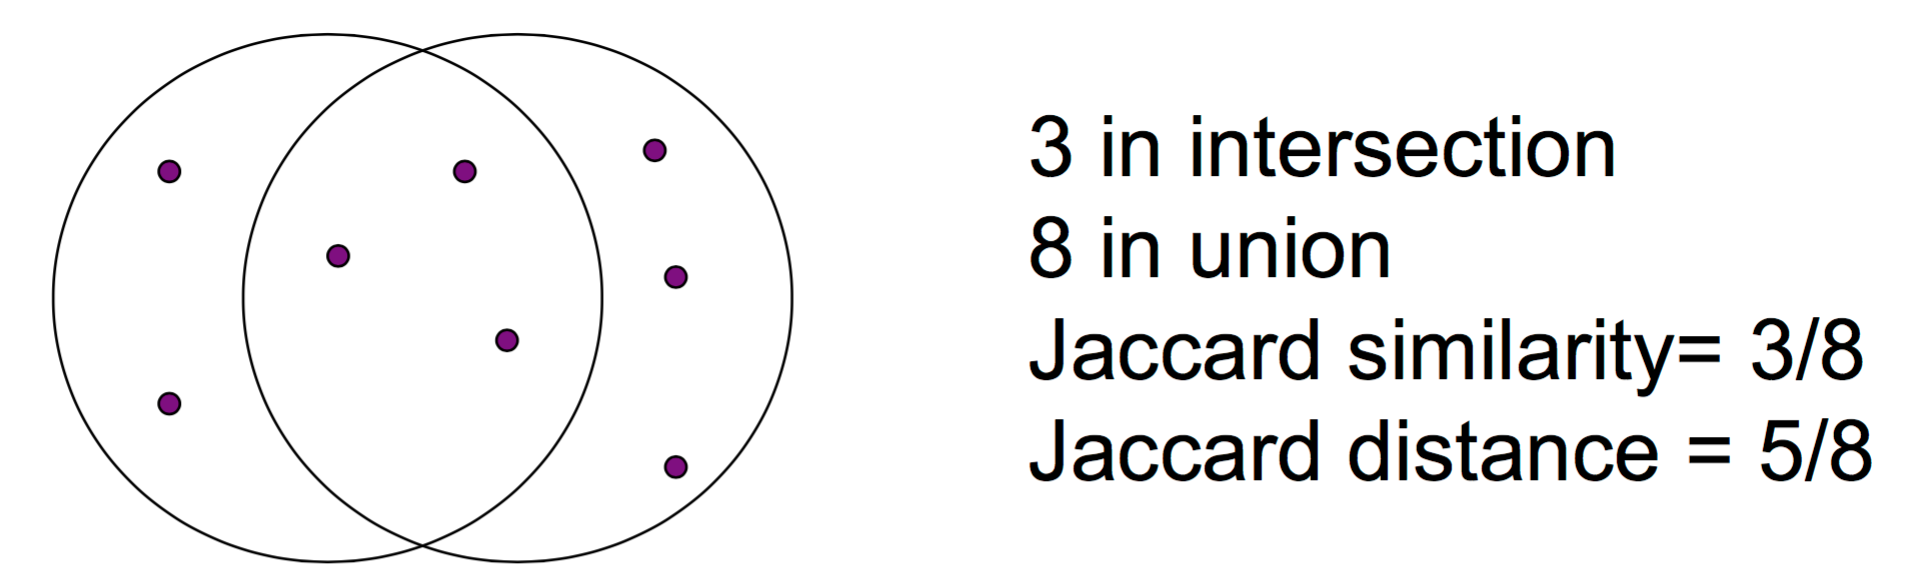
\includegraphics[width=10cm]{jaccard}
\end{frame}

%%%%%
  
\section{Finding Similar Items}

%%%%%
  
\begin{frame} \frametitle{Finding Similar Documents}

\begin{block}{Goal:}
Given a large number ($N$ in the millions or billions) of text documents, find pairs that are \emph{near duplicates}
\end{block}

\begin{block}{Applications:}
  \scriptsize
  \begin{itemize}
  \item Mirror websites, or approximate mirrors
    \begin{itemize}
    \item Don’t want to show both in a search
    \end{itemize}
  \item Similar news articles at many news sites
    \begin{itemize}
    \item Cluster articles by \emph{same story}
    \end{itemize}
  \end{itemize}
\end{block}
\begin{block}{Problems:}
  \scriptsize
  \begin{itemize}
  \item Many small pieces of one doc can appear out of order in another
  \item Too many docs to compare all pairs
  \item Docs are so large or so many that they cannot fit in main memory
  \end{itemize}
\end{block}
\end{frame}

%%%%%
  
\begin{frame} \frametitle{Three Essencial Steps}

\begin{enumerate}
\item \emph{Shingling:} Convert documents, emails, etc., to sets;

~\\

\item \emph{Minhashing:} Convert large sets to short signatures, while preserving similarity;
   \begin{itemize}
   \item Depends on the distance metric;
   \end{itemize}

~\\

\item \emph{Locality-sensitive hashing:} Focus on pairs of signatures likely to be from similar documents.
\end{enumerate}

\end{frame}

%%%%%
  
\begin{frame} \frametitle{The Big Picture}

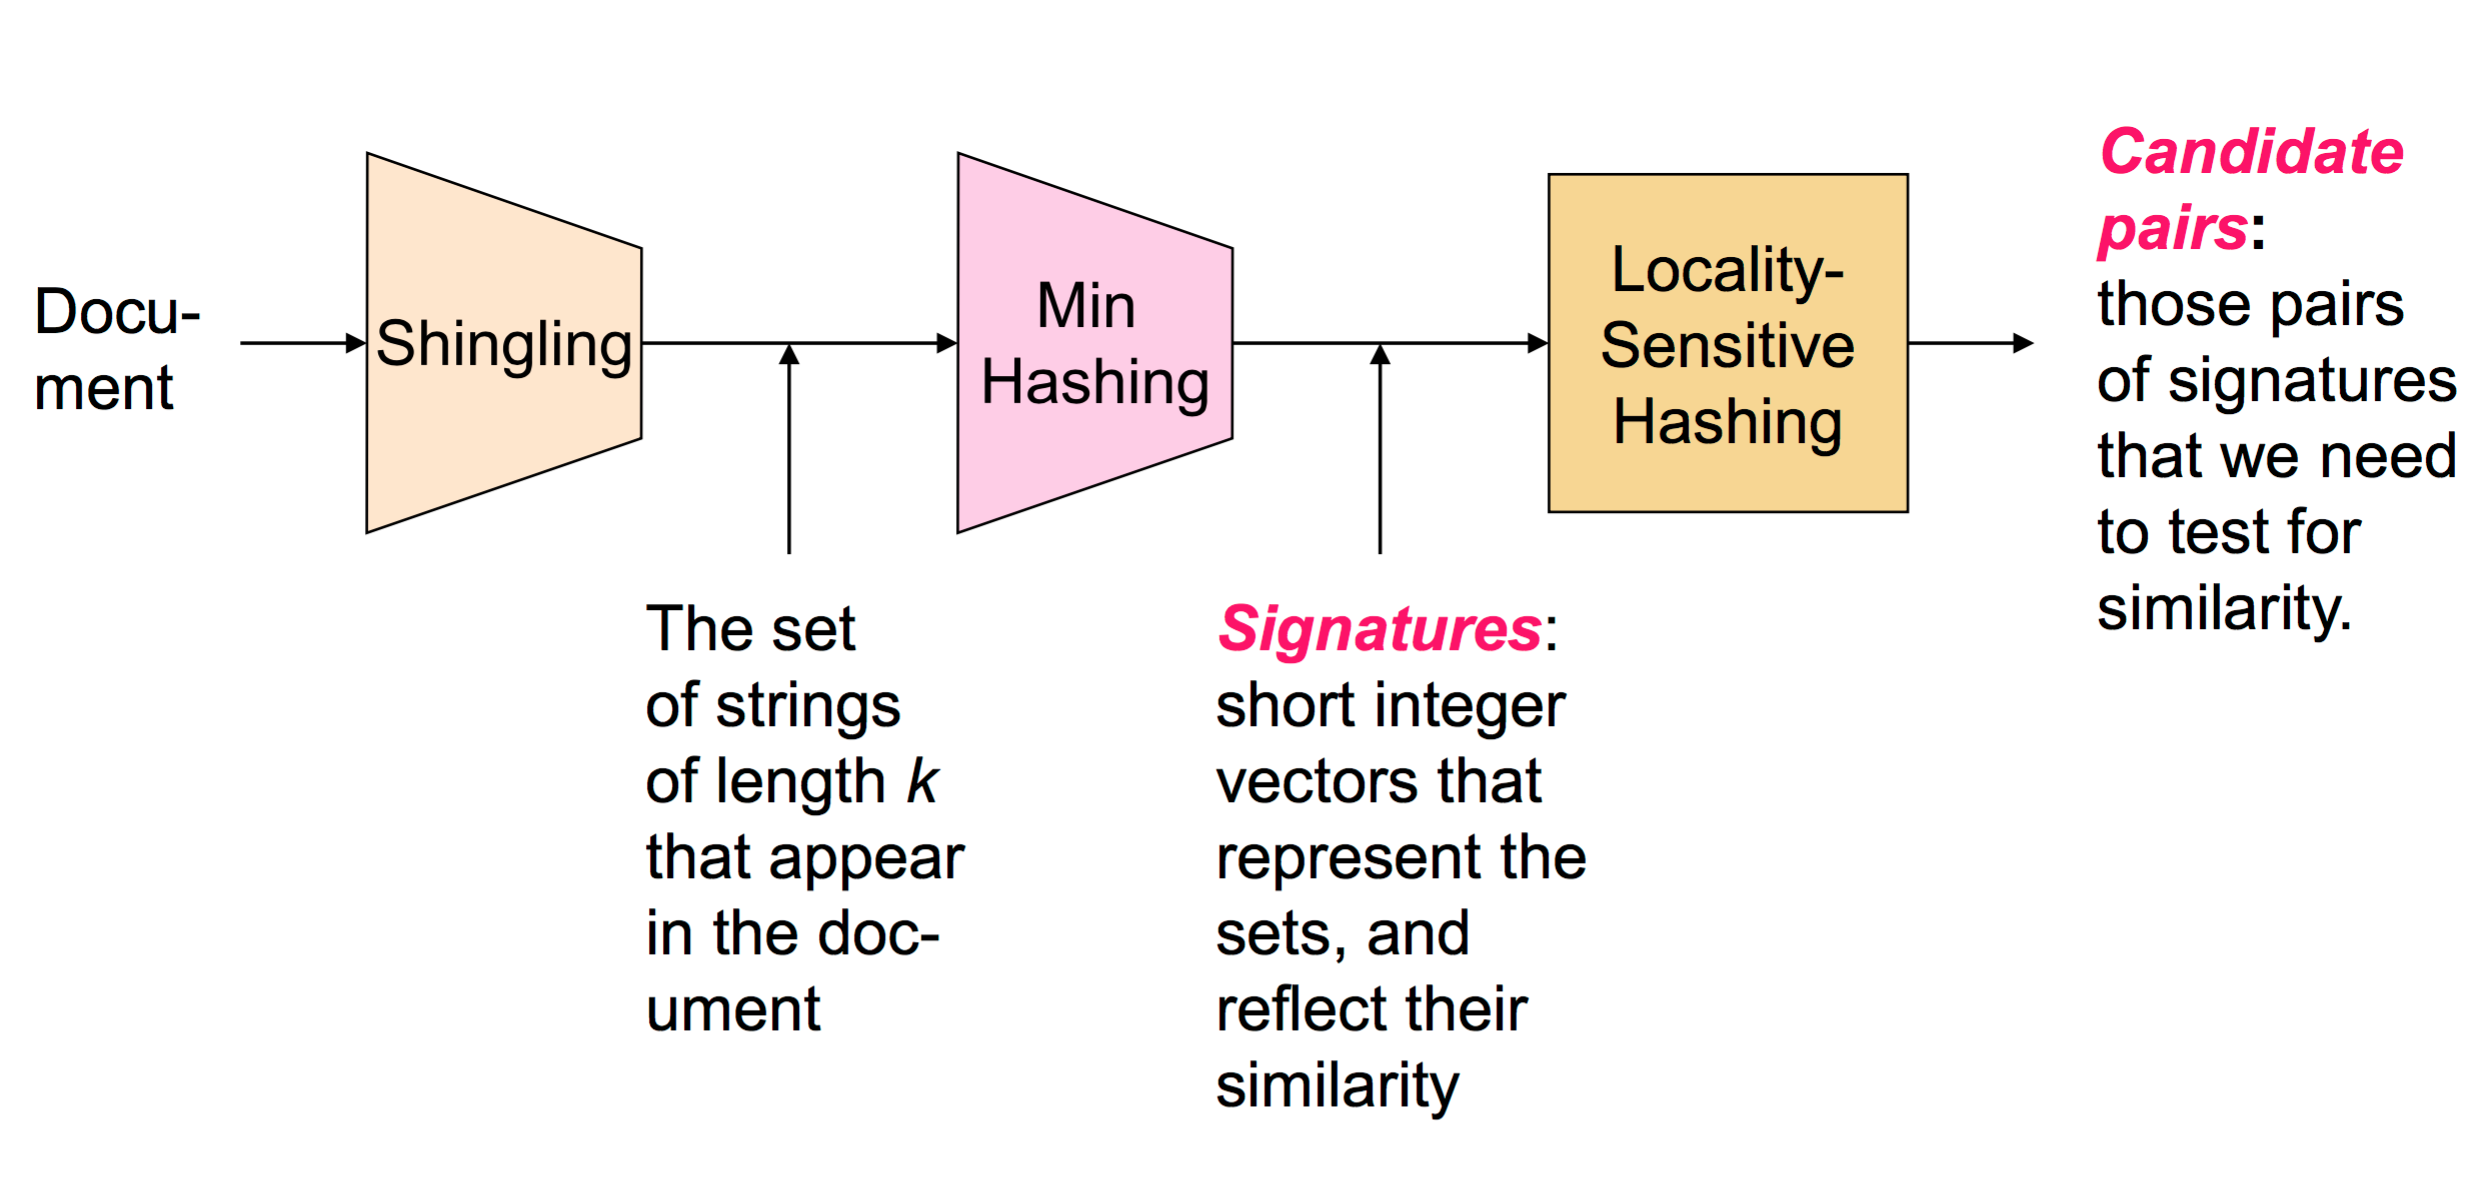
\includegraphics[width=10cm]{overall}

\end{frame}

%%%%%
  
\section{Shingles}

%%%%%
  
\begin{frame} \frametitle{Documents as High Dimensional Data}

\begin{block}{Step 1:}
Shingling: Convert documents, emails, etc., to sets
\end{block}

\begin{itemize}
\item Simple approaches...
   \begin{itemize}
   \item Document = set of words appearing in document
   \item Document = set of {\it important} words
   \end{itemize}
\item ...don’t work well for this application!
   \begin{itemize}
   \item Need to account for ordering of words
   \end{itemize}

\item A different way: \emph{Shingles}
\end{itemize}

\end{frame}

%%%%%
  
\begin{frame} \frametitle{Shingles}

\begin{itemize}
\item A $k$-shingle (or $k$-gram) for a document is a sequence of $k$ tokens that appears in the document
  \begin{itemize}
  \item Tokens can be characters, words or something else, depending on application
  \item Assume tokens = characters for next examples
  \end{itemize}
\end{itemize}

\begin{block}{Example: $k=2$; $D_1=abcab$}
  Set of 2-shingles: $S(D_1)=\{ab, bc, ca\}$
  
  ~\\
  Option: Shingles as a bag (i.e., multi-set), counting $ab$ twice
\end{block}
\begin{itemize}
\item Represent a doc by the set of hash values of its $k$-shingles
\end{itemize}

\end{frame}

%%%%%
  
\begin{frame} \frametitle{Compressing Shingles}

\begin{itemize}
\item To compress long shingles, we can hash them (e.g. 4 bytes)

\item Represent a doc by the set of hash values of its $k$-shingles

\item \emph{Idea:} Two documents could (rarely) appear to have shingles in common, when in fact only the hash-values were shared
\end{itemize}

\begin{block}{Example: $k=2$; $D_1=abcab$}
  Set of 2-shingles: $S(D_1)=\{ab, bc, ca\}$
  
  ~\\
  Hash the shingles: $h(D_1)=\{1, 5, 7\}$
\end{block}
\end{frame}

%%%%%
  
\begin{frame} \frametitle{Similarity Metric for Shingles}

\begin{itemize}
\item Document $D_1$ = set of $k$-shingles $C_1=S(D_1)$
\item Equivalently, each document is a 0/1 vector in the space of $k$-shingles
   \begin{itemize}
   \item Each unique shingle is a dimension
   \item Vectors are very sparse
   \end{itemize}
\item A natural similarity measure is the Jaccard similarity:
\end{itemize}

\begin{block}{}
\begin{center}
$Sim(C_1, C_2) = \frac{|C_1 \cap C_2|}{|C_1 \cup C_2|}$
\end{center}
\end{block}
\end{frame}

%%%%%
  
\begin{frame} \frametitle{Working Assumption}

\begin{itemize}
\item Documents that have lots of shingles in common have similar text, even if the text appears in different order

~\\

\item \emph{Careful:} You must pick $k$ large enough, or most documents will have most shingles
   \begin{itemize}
   \item $k = 5$ is OK for short documents
   \item $k = 10$ is better for long documents
   \end{itemize}
\end{itemize}
\end{frame}

%%%%%
  
\begin{frame} \frametitle{Motivation for Minhash/LSH}

\begin{itemize}
\item Suppose we need to find near-duplicate documents among $N=1$ million documents

\item Naively, we'd have to compute pairwaise Jaccard similarites for every pair of docs
\begin{itemize}
  \item i.e, $\frac{N \ times (N-1)}{2} ≈ 5 \times 10^{11}$ comparisons
  \item At 10^5 secs/day and 10^6 comparisons/sec, it would take 5 days
\end{itemize}

\item For $N = 10$ million, it takes more than a year...
\end{itemize}
\end{frame}

\section{Minhashing}

%%%%%
  
\begin{frame} \frametitle{The Big Picture}
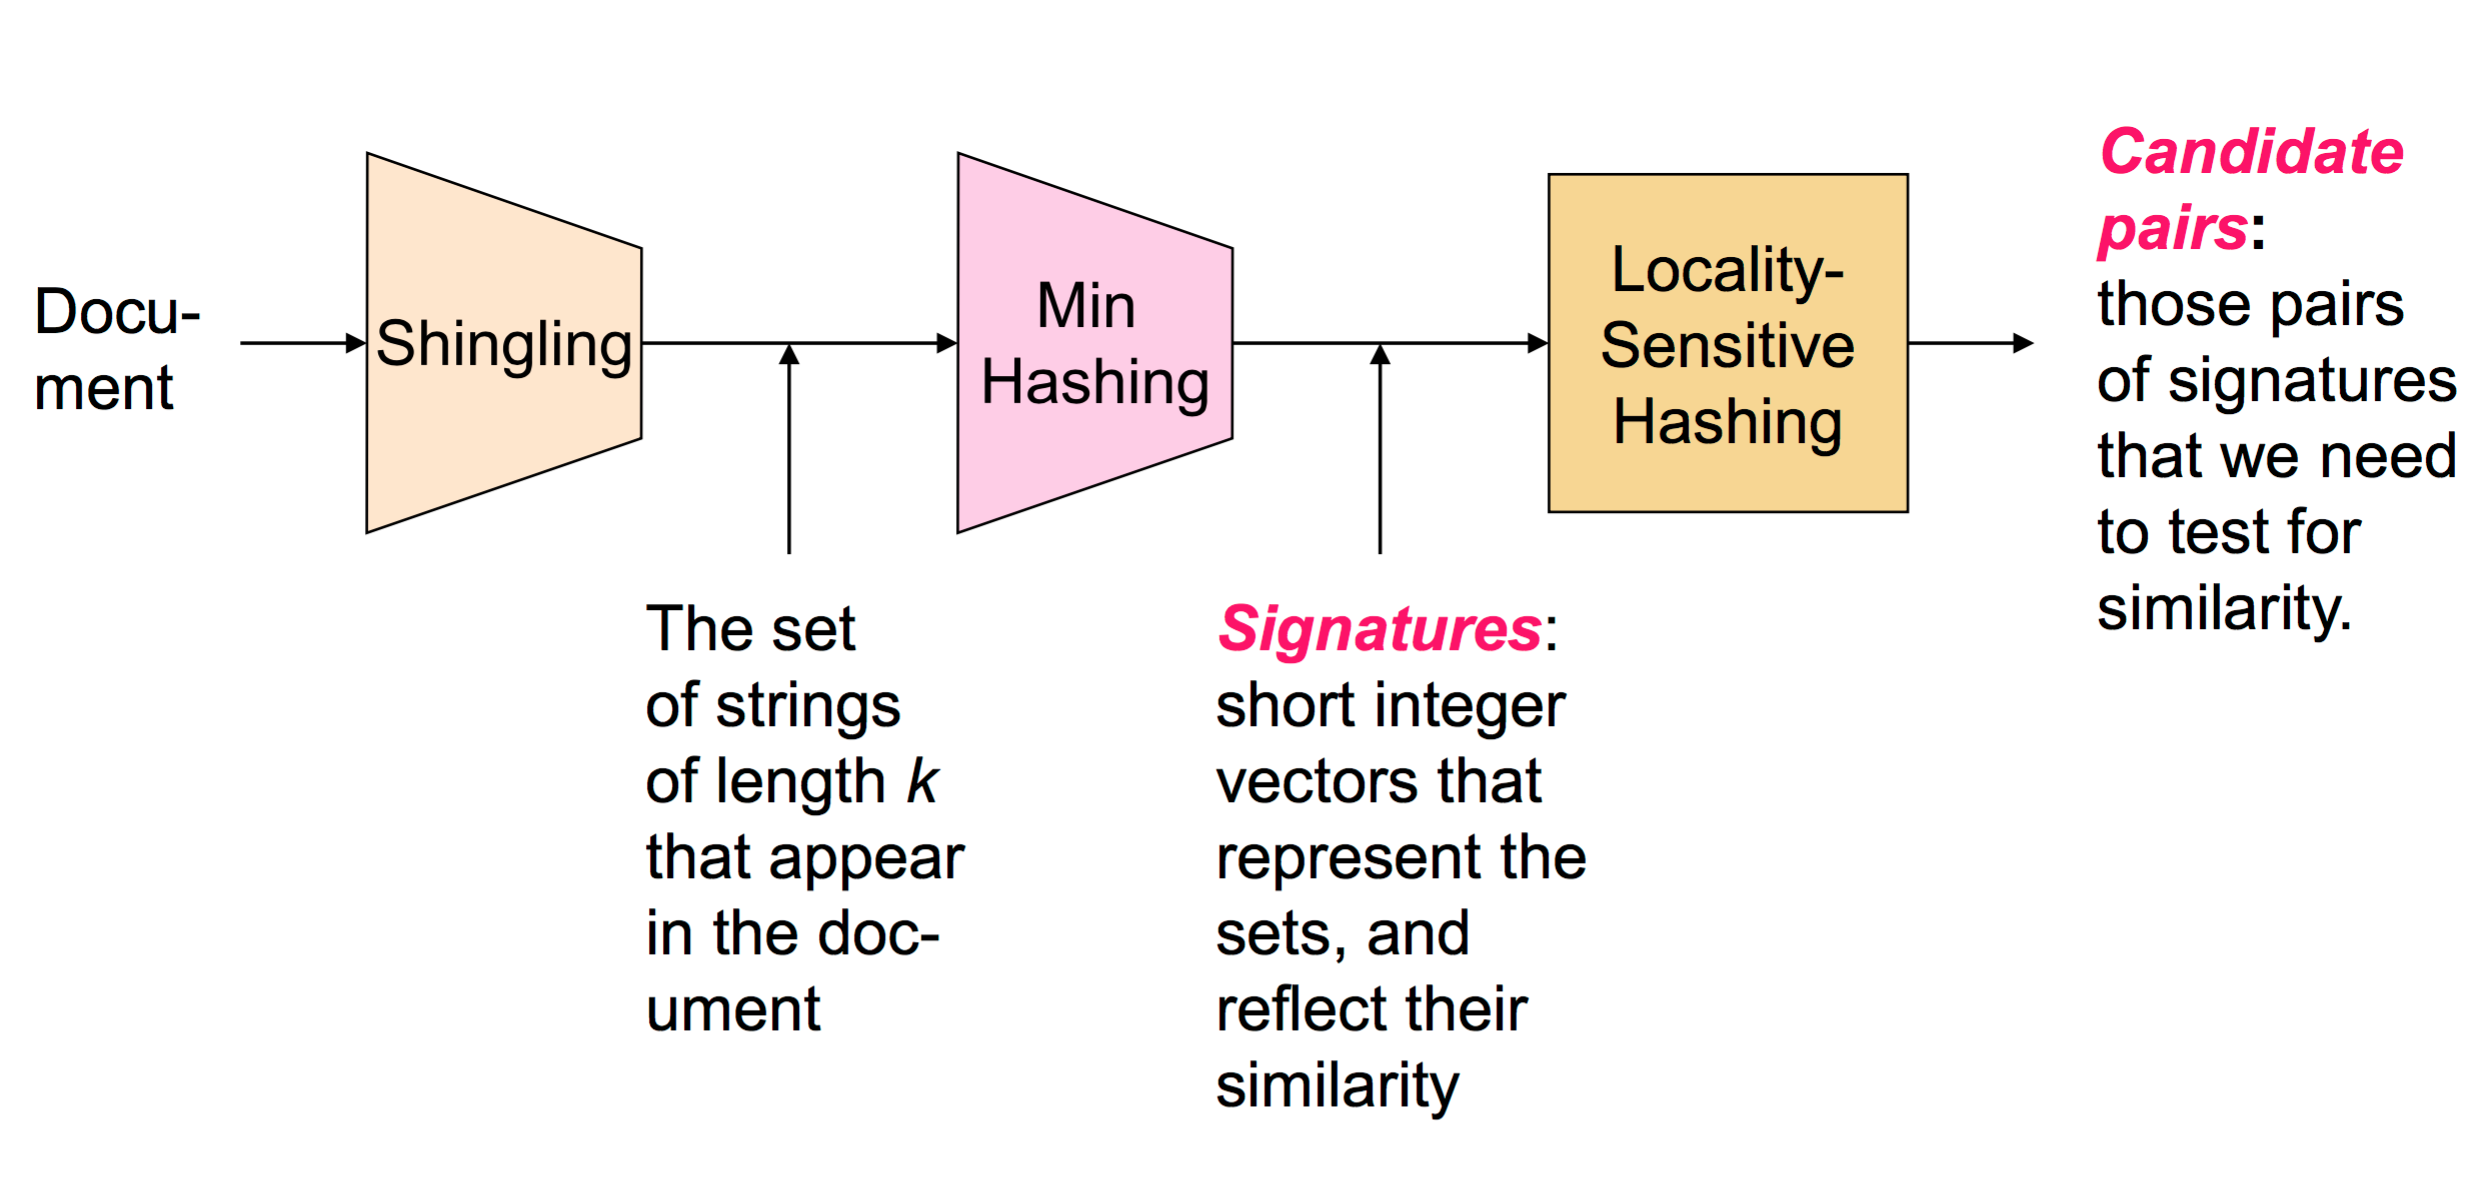
\includegraphics[width=10cm]{overall}
\end{frame}

%%%%%
  
\begin{frame} \frametitle{Encoding Sets as Bit Vectors}

\begin{block}{}
Many similarity problems can be formalized as finding subsets hat have significant intersection

\begin{itemize}
\item Encode sets using 0/1 (bit, Boolean) vectors
\item One dimension per element in the universal set
\item Interpret set intersection as bitwise AND, and set union as bitwise OR
\end{itemize}
\end{block}

\begin{block}{Example: $C_1 = 10111$; $C_2 = 10011$}
  \begin{itemize}
  \item Size of intersection = 3; 
  \item Size of union = 4
  \item Jaccard similarity (not distance) = 3/4
  \item $d(C_1,C_2) = 1 –$ (Jaccard similarity) = 1/4
  \end{itemize}
\end{block}  
\end{frame}

%%%%%
  
\begin{frame} \frametitle{From Sets to Boolean Matrices}

 \begin{columns}[T]
    \begin{column}{0.7\textwidth}
\begin{itemize}
\item Rows = elements of the universal set
\item Columns = sets
\item 1 in row $e$ and column $s$ if and only if $e$ is a member of $s$
\item Column similarity is the Jaccard similarity of the sets of their rows with 1
\item Typical matrix is sparse
\end{itemize}
  \end{column}
  \begin{column}{0.25\textwidth}
   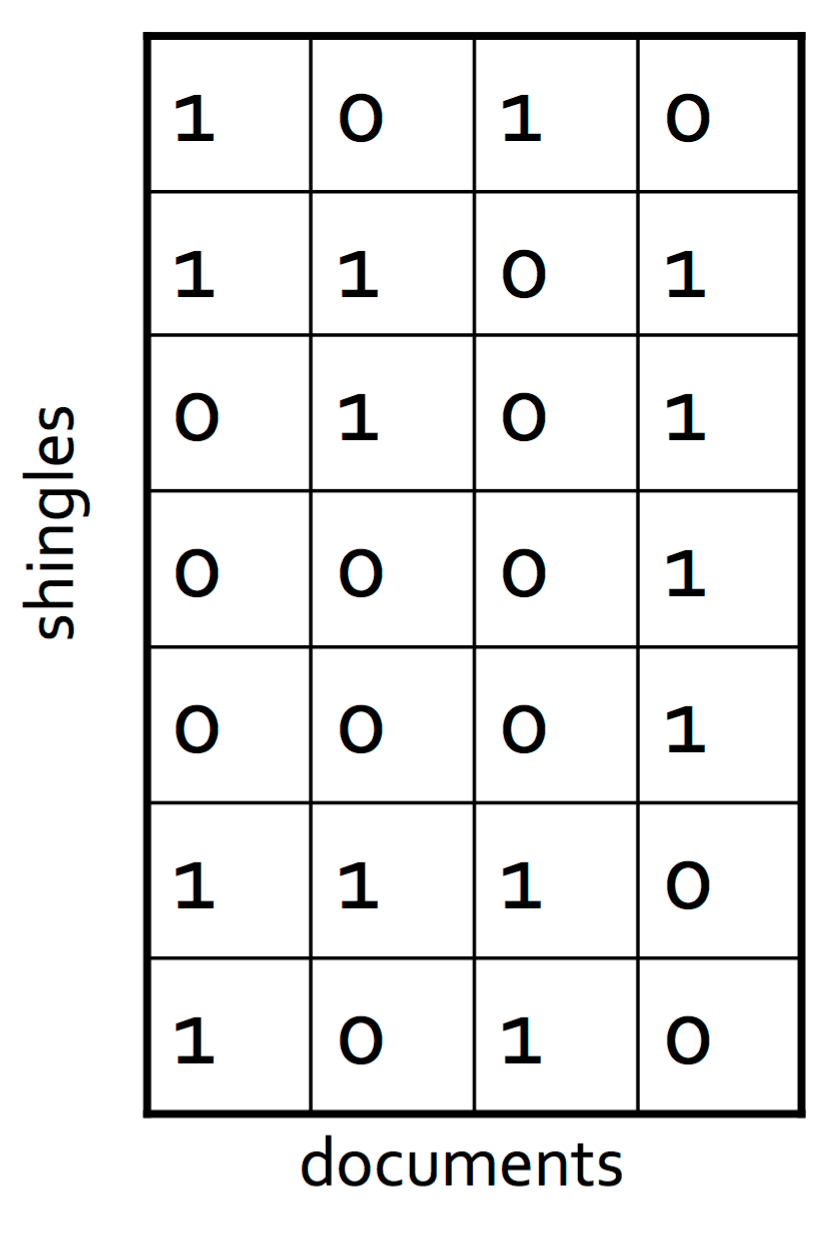
\includegraphics[width=5cm]{matrix}
  \end{column}
 \end{columns}
\end{frame}

%%%%%
  
\begin{frame} \frametitle{Jaccard of Columns}

 \begin{columns}[T]
    \begin{column}{0.7\textwidth}
\begin{itemize}
\item Each document is a column:

  \begin{block}{Example: $C1 = 1100011; C2 = 0110010$}
  \begin{itemize}
  \item Size of intersection = 2; 
  \item size of union = 5, 
  \item Jaccard similarity (not distance) = 2/5
  \item $d(C_1,C_2) = 1 –$ (Jaccard similarity) = 3/5
  \end{itemize}
  \end{block}  

\item We might not really represent the data by a boolean matrix
  \begin{itemize}
  \item Sparse matrices are usually better represented by the list of places where there is a non-zero value
  \end{itemize}
\end{itemize}
  \end{column}
  \begin{column}{0.25\textwidth}
   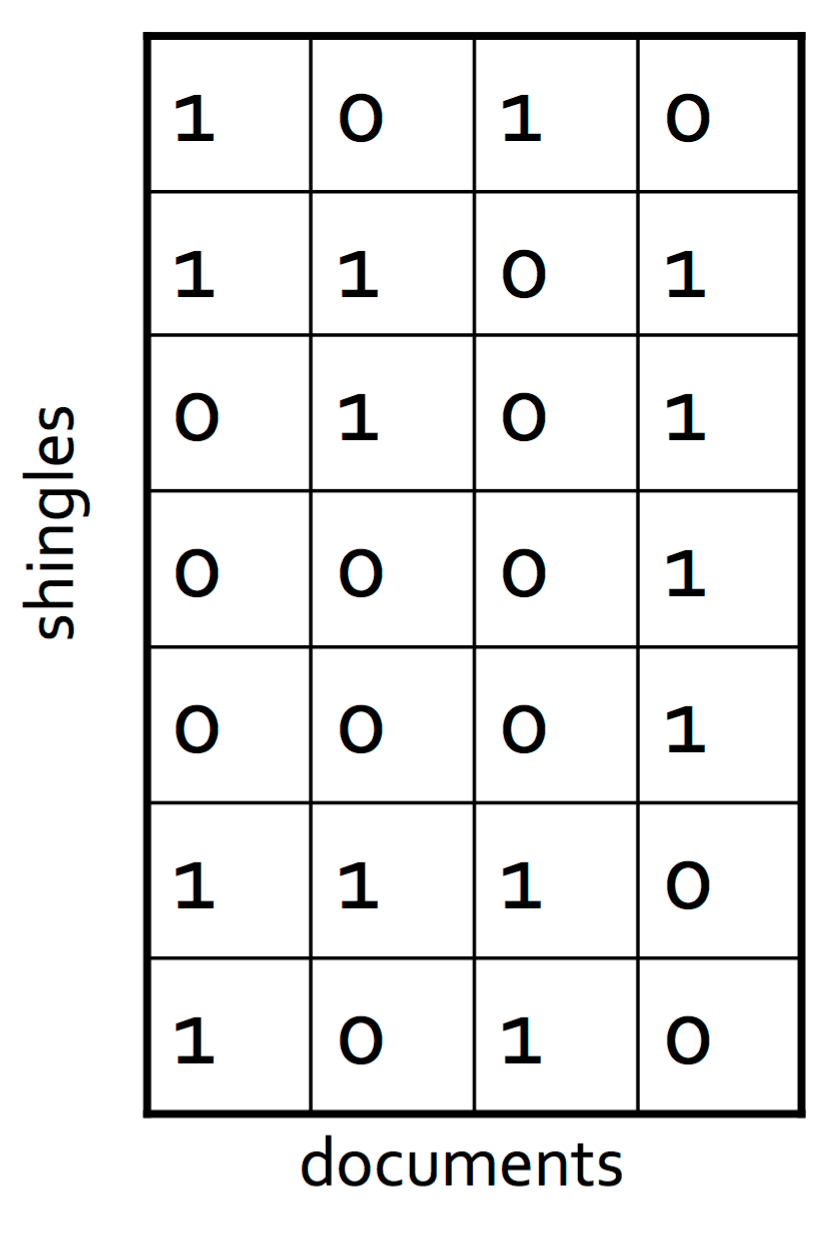
\includegraphics[width=5cm]{matrix}
  \end{column}
 \end{columns}

\end{frame}

%%%%%
  
\begin{frame} \frametitle{Finding Similar Columns}
So far:
  Documents represented as sets of shingles
  Represent sets as boolean vectors in a matrix

Next Goal: Find similar columns
 1) Signatures of columns: small summaries of columns
 2) Examine pairs of signatures to find similar columns 
       Essential that similarities of signatures and columns are related
 3) Optional: check that columns with similar signatures are really similar

Warnings:
  Comparing all pairs may take too much time: job for LSH
  These methods can produce false negatives, and even false positives (if the optional check is not made)
  \end{frame}

%%%%%
  
\begin{frame} \frametitle{Signatures of Columns}

Key idea: \emph{hash} each column $C$ to a small signature $h(C)$, such that:
  (1) $h(C)$ is small enough that the signature fits in RAM
  (2) $sim(C_1, C_2)$ is the same as the similarity of signatures $h(C_1)$ and $h(C_2)$

Goal: Find a hash function h() such that:
  if $sim(C_1,C_2)$ is high, then with high prob. $h(C_1) = h(C_2)$
  if $sim(C_1,C_2)$ is low, then with high prob. $h(C_1) \neq h(C_2)$

Hash docs into buckets, and expect that most pairs of near duplicate docs hash into the same bucket
\end{frame}

%%%%%
  
\begin{frame} \frametitle{Min-Hashing (1)}

Goal: Find a hash function h() such that:
  if sim(C1,C2) is high, then with high prob. $h(C1) = h(C2)$
  if sim(C1,C2) is low, then with high prob. $h(C1) \neq h(C2)$

Clearly, the hash function depends on the similarity metric:
  Not all similarity metrics have a suitable hash function
  There is a suitable hash function for Jaccard similarity: Min-hashing
  
\end{frame}

%%%%%
  
\begin{frame} \frametitle{Min-Hashing (2)}

Imagine the rows of the boolean matrix permuted under random permutation $\pi$
Define a hash function $h_\pi(C)$ = the number of the first (in the permuted order $\pi$) row in which column C has value 1:
  $h_\pi (C) = \min_\pi(C)$
Use several (e.g., 100) independent hash functions (i.e., permutations) to create a signature of a column

\end{frame}

%%%%%
  
\begin{frame} \frametitle{Min-Hashing (3)}

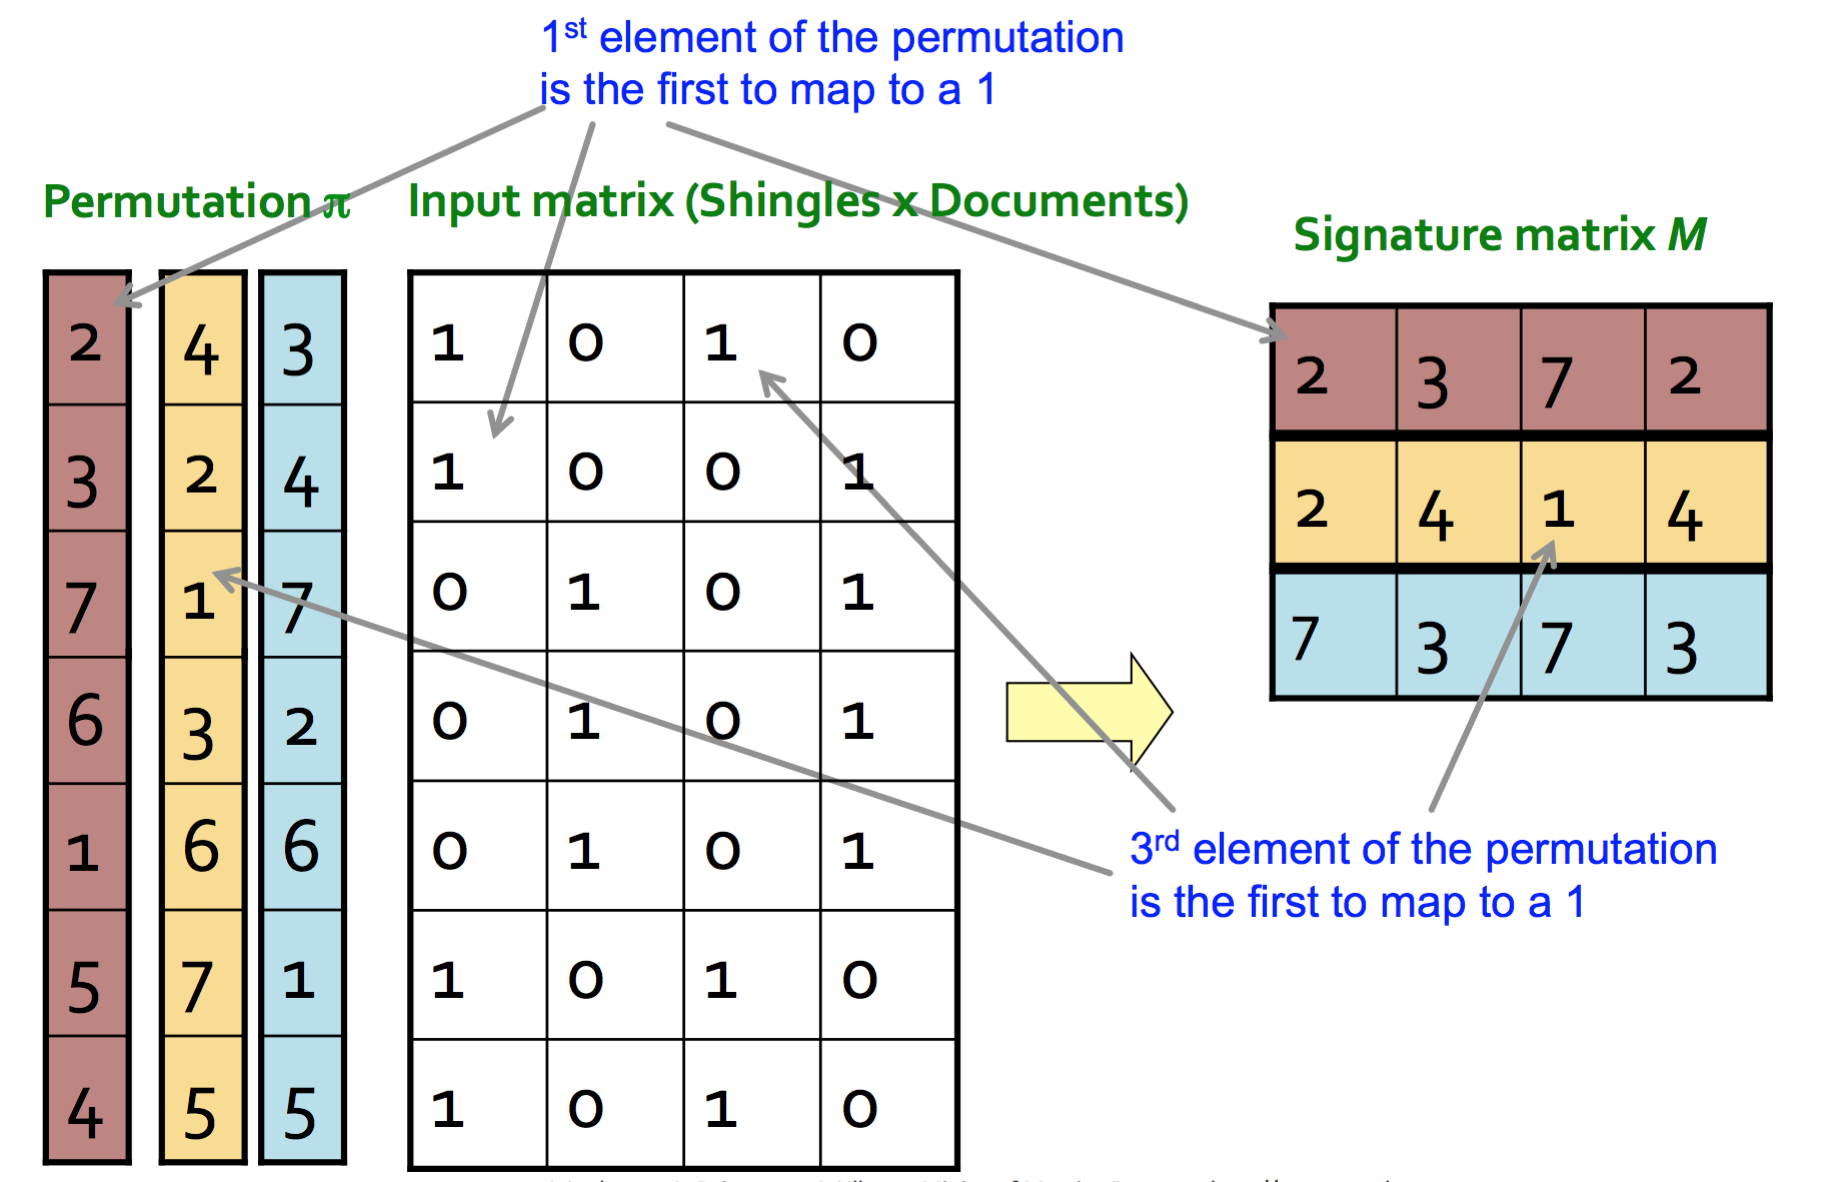
\includegraphics[width=10cm]{minhash}

\end{frame}

%%%%%
  
\begin{frame} \frametitle{Surprising Property}

Under a random permutation $\pi$, $Pr[h_\pi(C_1) = h_\pi(C_2)] = sim(C_1, C_2)$

%Let X be a set of shingles, X ⊆ [2^{64}], x∈X
%Then: Pr[π(y) = min(π(X))] = 1/|X|
%  It is equally likely that any y∈X is mapped to the min element
%Let x be s.t. \pi(x) = min(\pi(C1∪C2))
%Then either \pi(x) = min(\pi(C1)) if x \in C1 , or \pi(x) = \min(\pi(C2)) if x \in C2
%So the probability that both are true is the probability x \in C1 \cap C2
%Pr[min(\pi(C1))=min(\pi(C2))]=|C1 \cap C2|/|C1 \cup C2|= sim(C1, C2)
\end{frame}

%%%%%
  
\begin{frame} \frametitle{Similarity for Signatures}

We know $Pr[h_\pi(C_1) = h_\pi(C_2)] = sim(C_1, C_2)$
Now generalize to multiple hash functions
The similarity of two signatures is the fraction of the hash functions in which they agree
Note: Because of the minhash property, the similarity of columns is the same as the expected similarity of their signatures

\end{frame}

%%%%%
  
\begin{frame} \frametitle{Example}

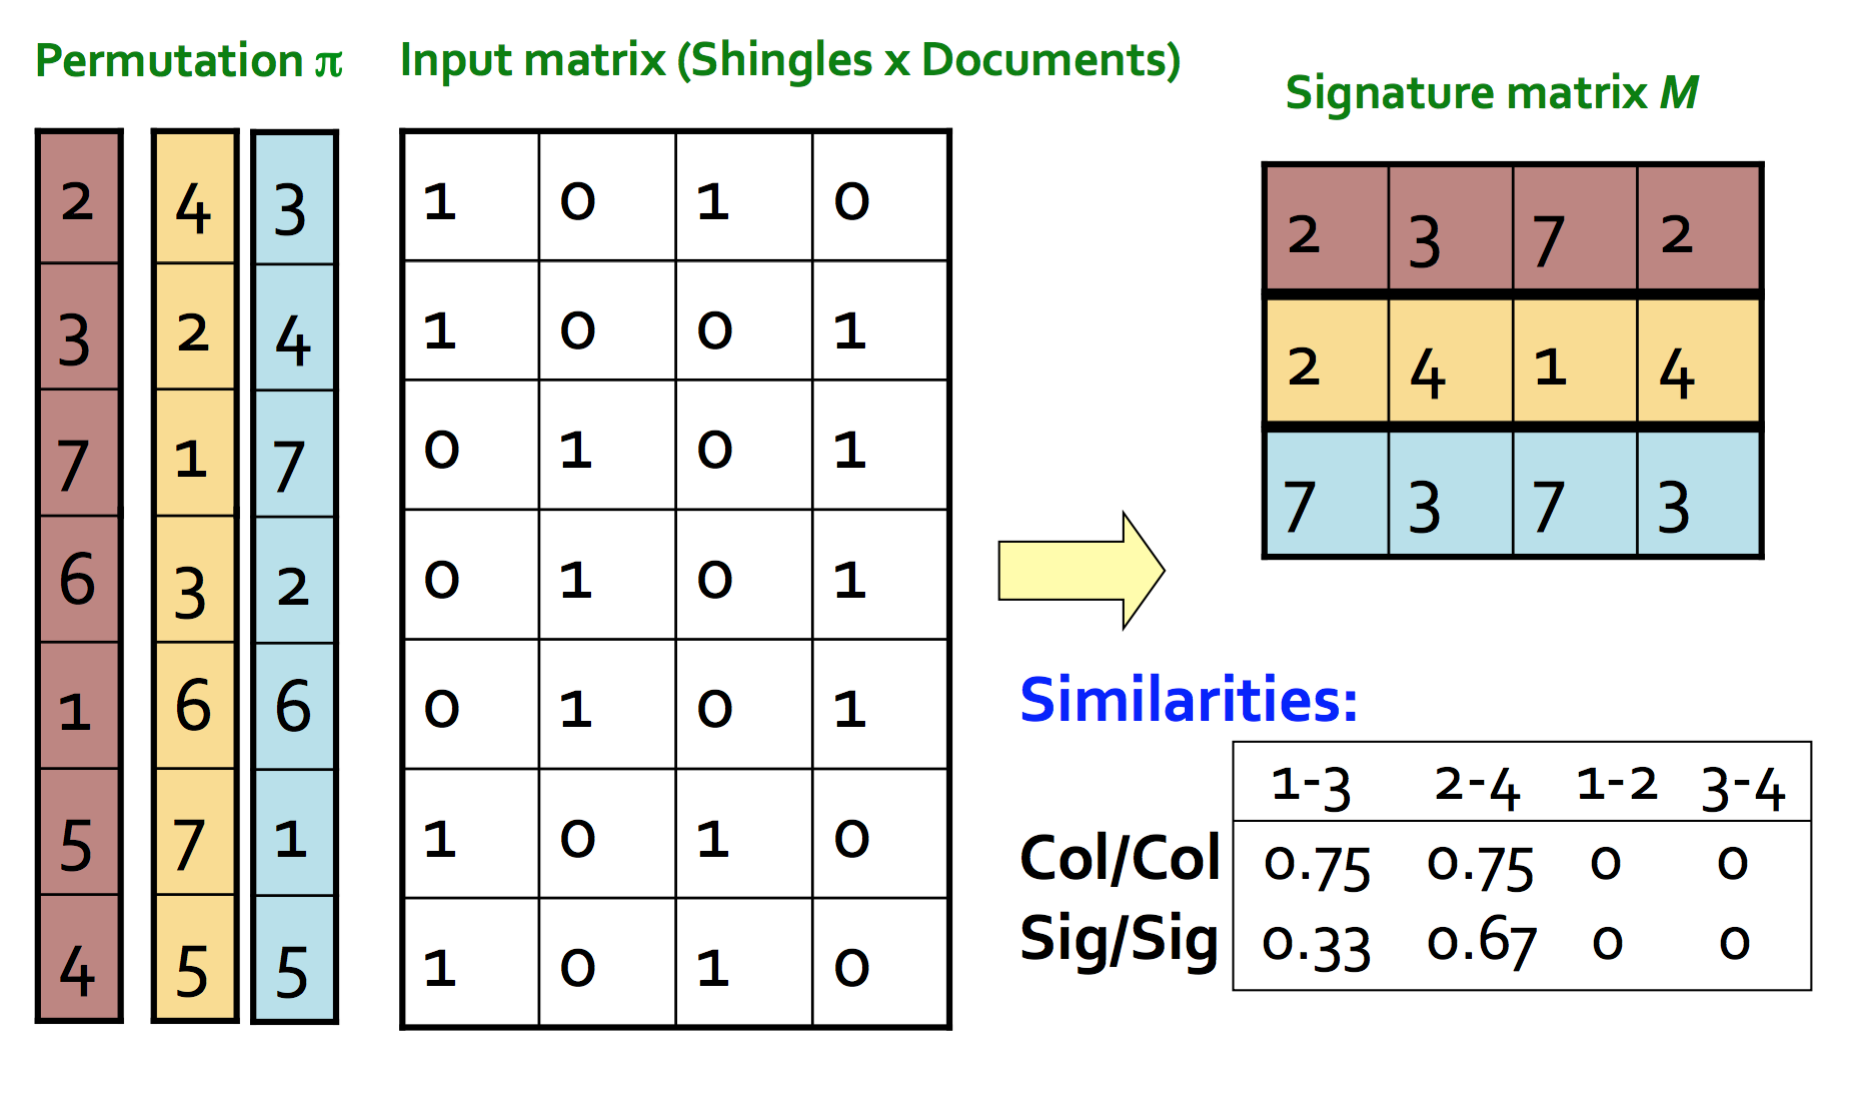
\includegraphics[width=10cm]{example}

\end{frame}

%%%%%
  
\begin{frame} \frametitle{Minhash Signatures}

Pick 100 random permutations of the rows
Think of $sig(C)$ as a column vector
Let $sig(C)[i]$ = according to the $i$-th permutation, the index of the first row that has a 1 in column C
   $sig(C)[i] = min (\pi_i(C))$
Note: The sketch (signature) of document C is small -- \~100 bytes!
We achieved the goal of \emph{compressing} long bit vectors into short signatures

\end{frame}

%%%%%
  
\section{Locality-sensitive hashing}

%%%%%
  
\begin{frame} \frametitle{The Big Picture}

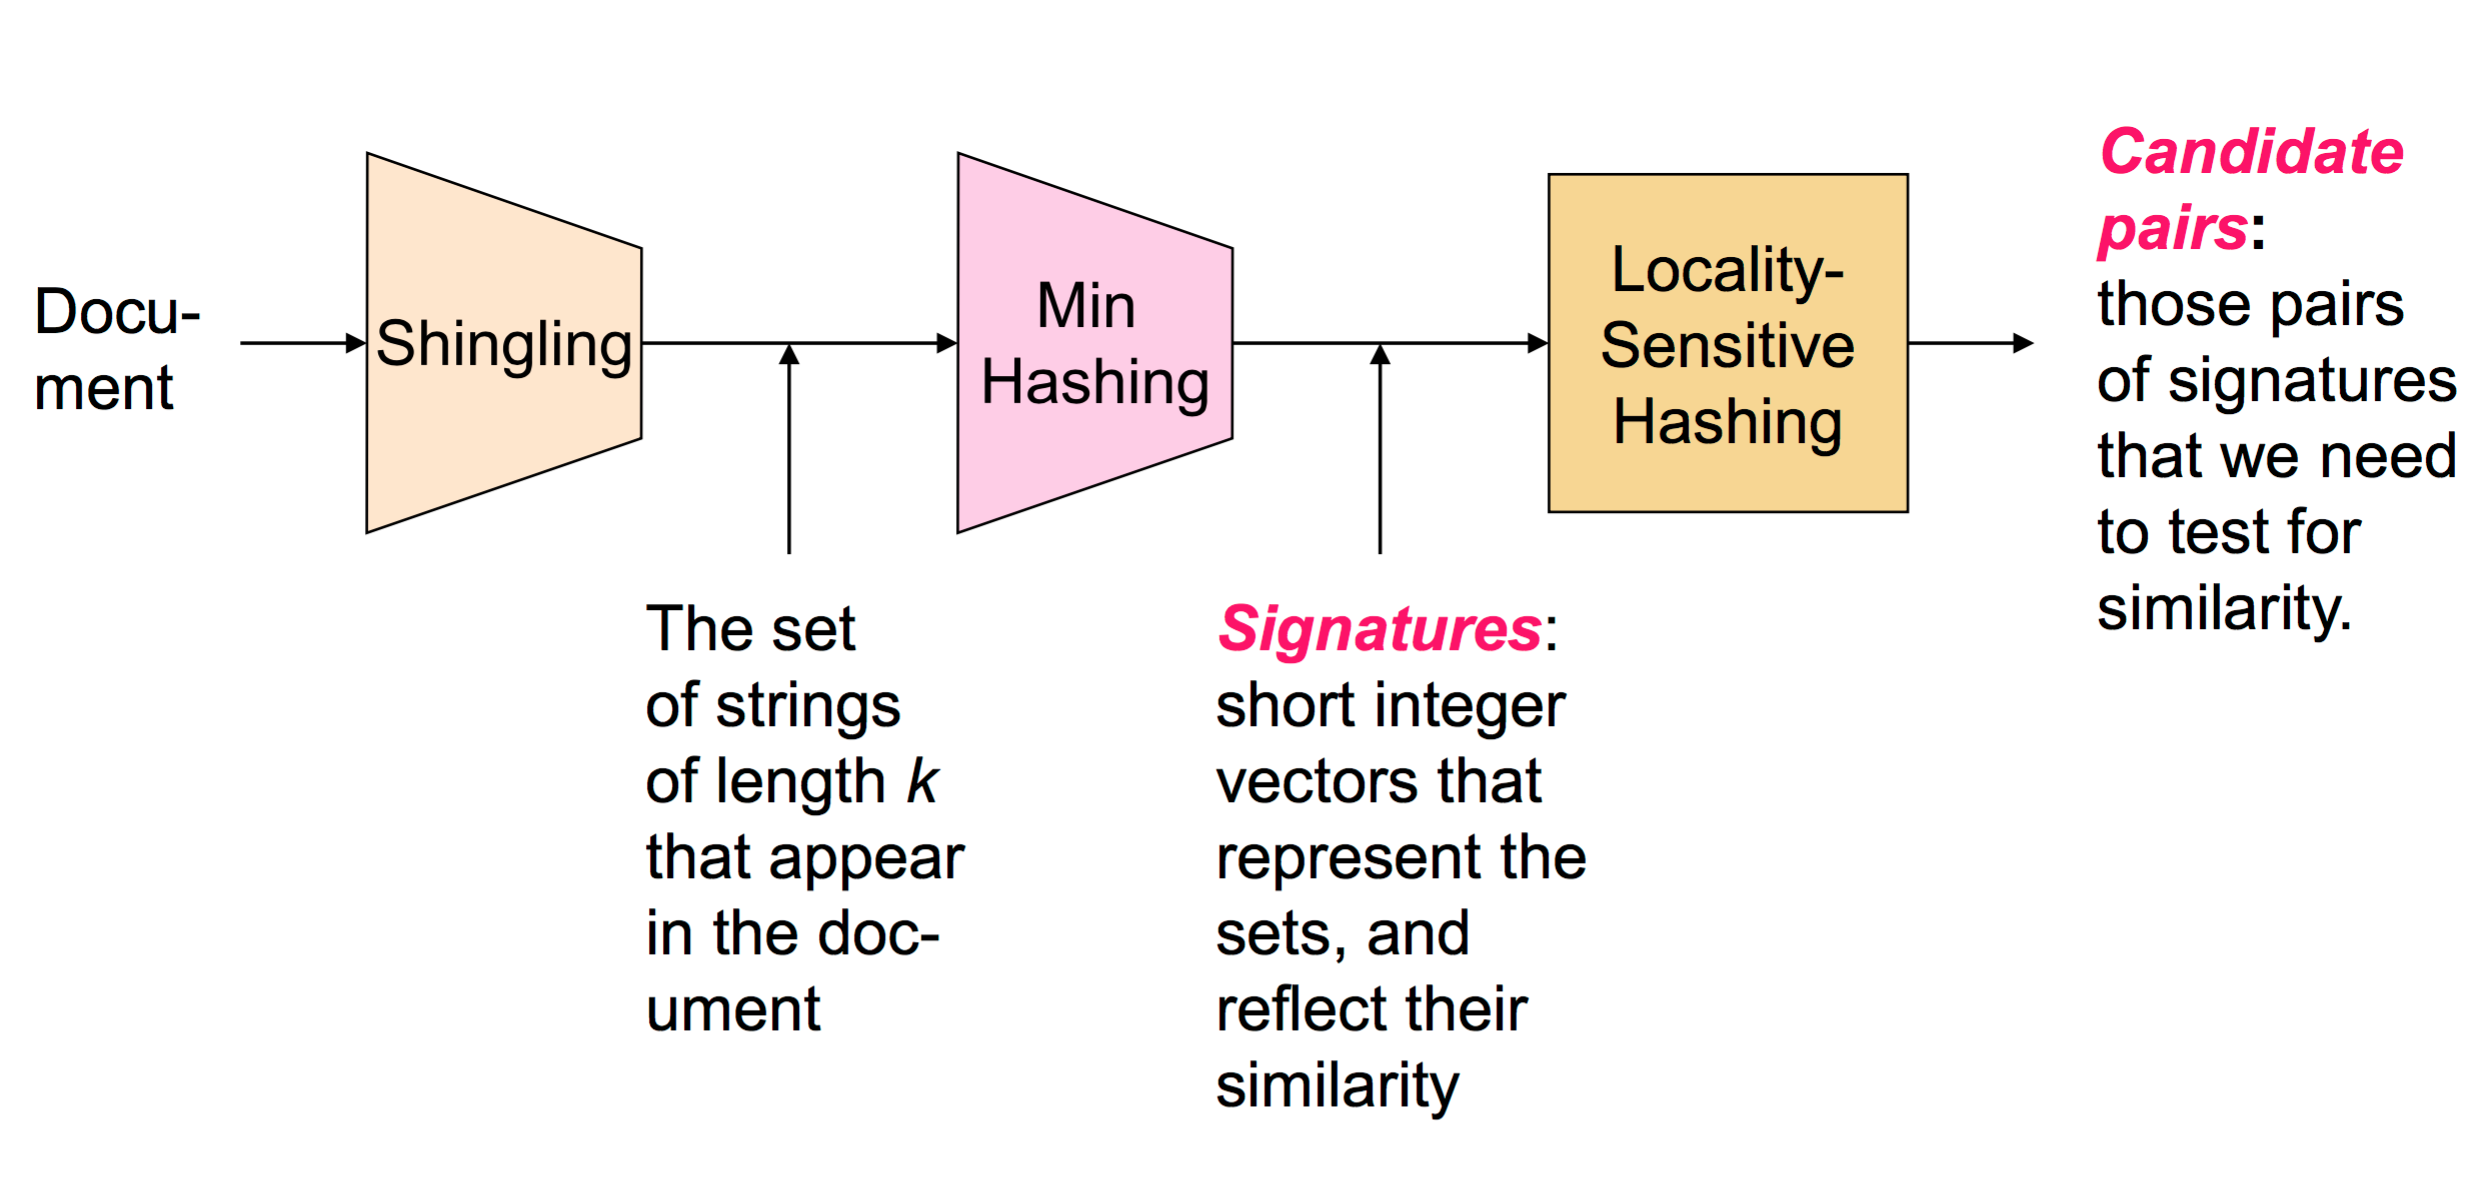
\includegraphics[width=10cm]{overall}

\end{frame}

%%%%%
  
\begin{frame} \frametitle{LSH : General Intuition}

Goal: Find documents with Jaccard similarity at least s (for some similarity threshold, e.g., s=0.8)
LSH -- Use a function f(x,y) that tells whether x and y is a candidate pair, i.e. a pair of elements whose similarity must be evaluated
For minhash matrices:
  Hash columns of signature matrix M to many buckets
  Each pair of documents that hashes into the same bucket is a candidate pair
  
\end{frame}

%%%%%
  
\begin{frame} \frametitle{Candidates from Minhash}

Pick a similarity threshold s, a fraction < 1
Columns x and y of M are a candidate pair if their signatures agree on at least fraction s of their rows: 

M (i, x) = M (i, y) for at least fraction s values of i

We expect documents x and y to have the same similarity as their signatures

\end{frame}

%%%%%
  
\begin{frame} \frametitle{LSH for Minhash Signatures}

Big idea: Hash columns of signature matrix M several times
Arrange that (only) similar columns are likely to hash to the same bucket, with high probability
Candidate pairs are those that hash to the same bucket

\end{frame}

%%%%%
  
\begin{frame} \frametitle{Partition M into Bands (1)}

Divide matrix $M$ into b bands of $r$ rows
For each band, hash its portion of each column to a hash table with $k$ buckets
Make $k$ as large as possible
Candidate column pairs are those that hash to the same bucket for 1 band or more
Tune $b$ and $r$ to catch most similar pairs, but few non-similar pairs

\end{frame}

%%%%%
  
\begin{frame} \frametitle{Partition M into Bands (2)}

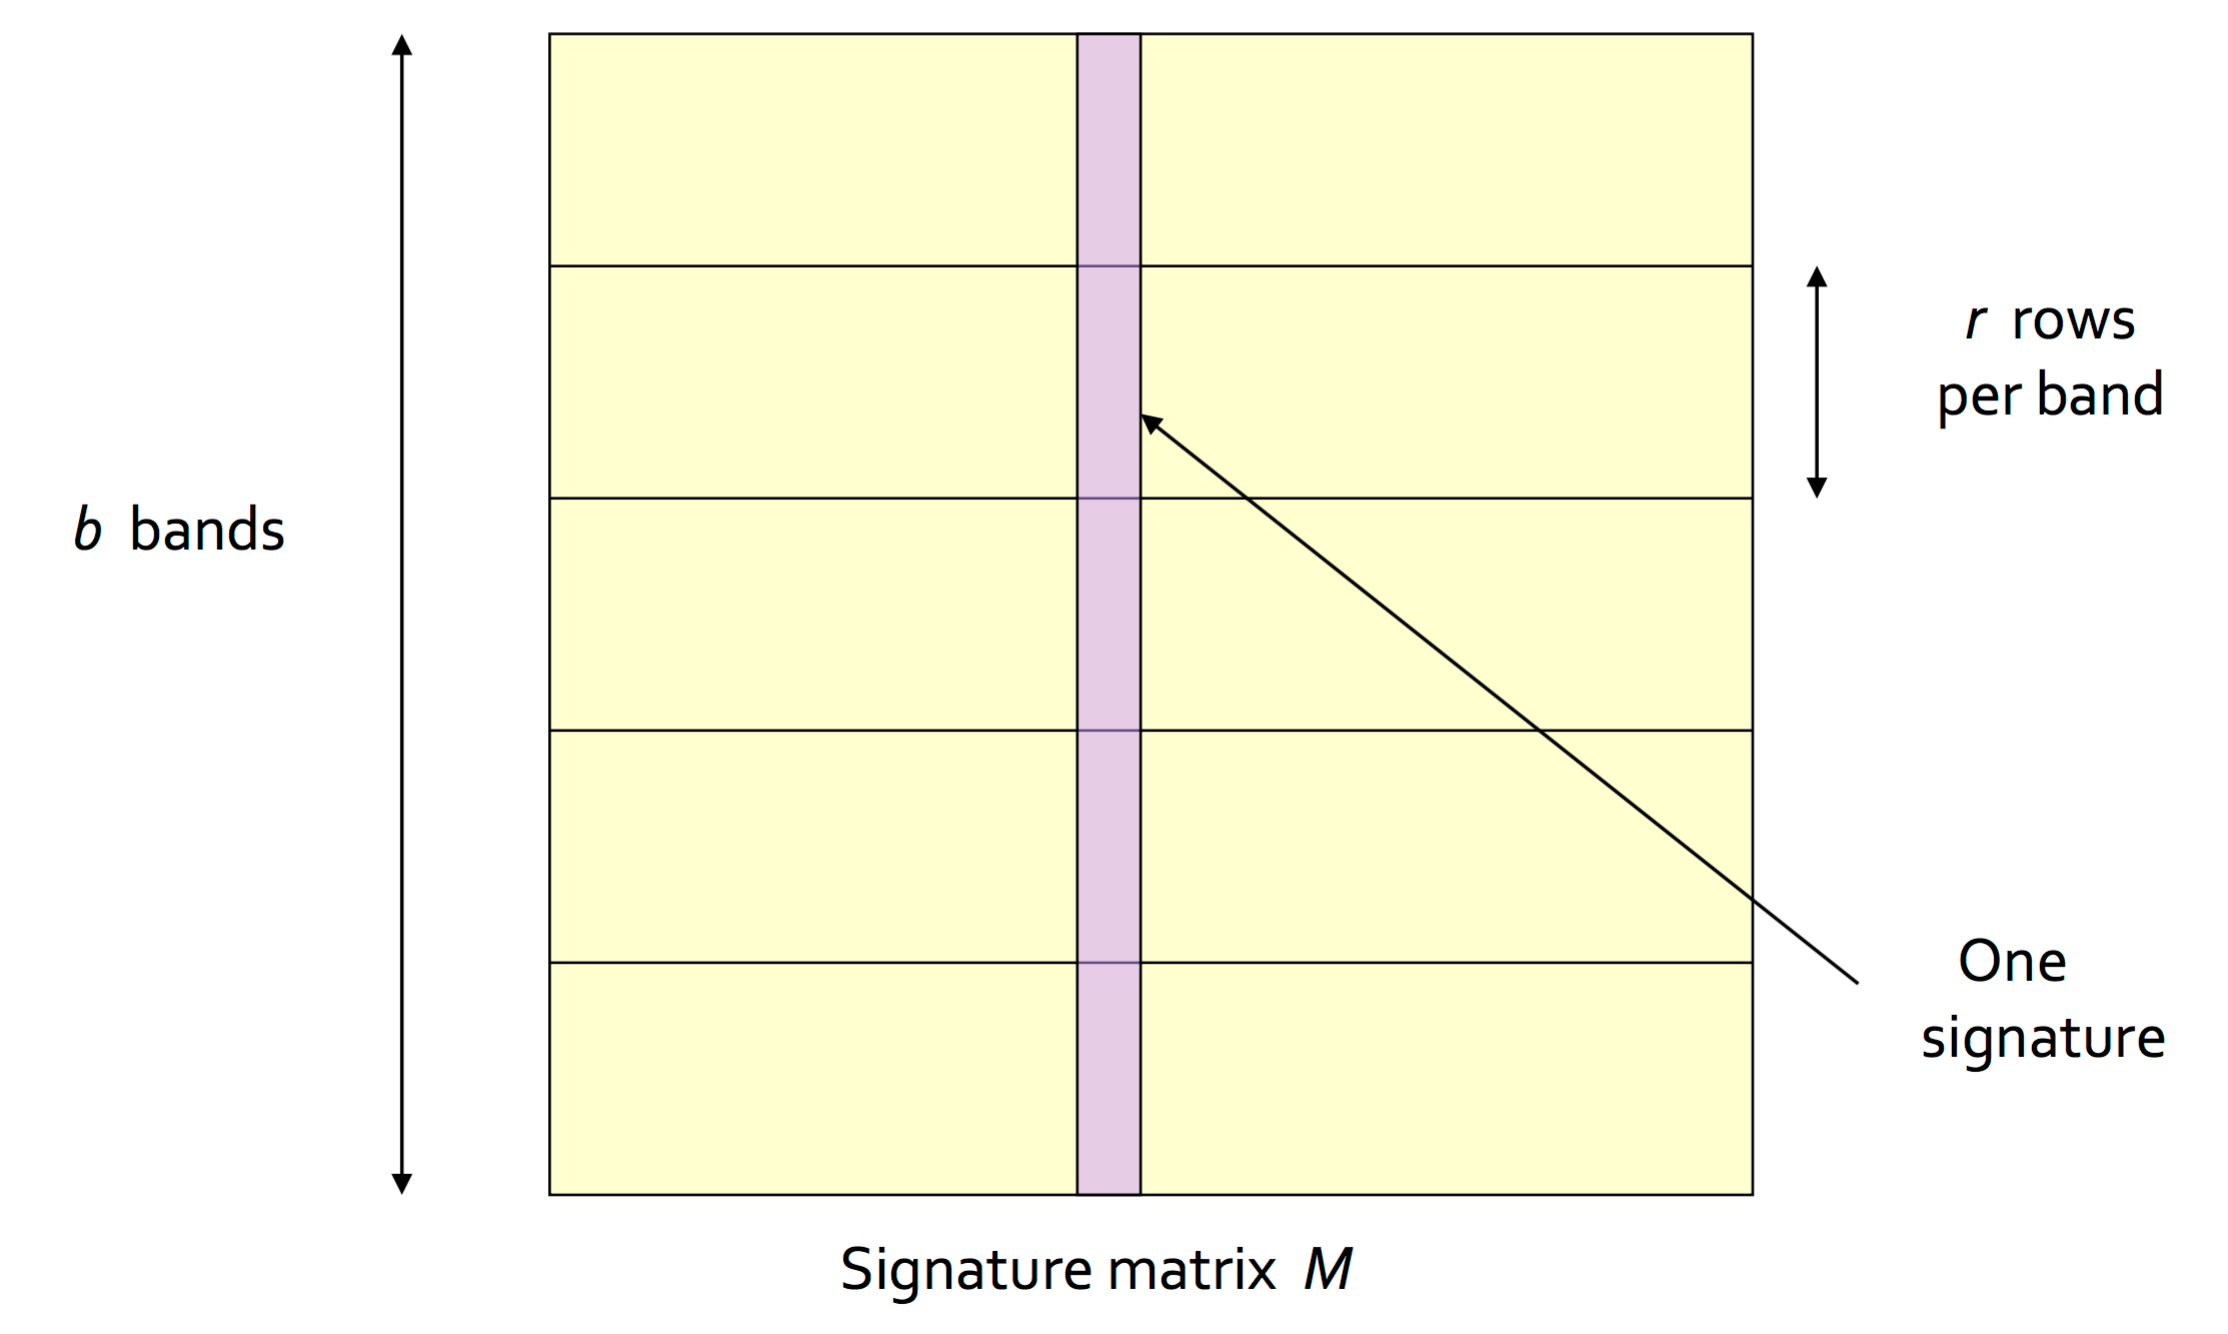
\includegraphics[width=10cm]{bands}

\end{frame}

%%%%%
  
\begin{frame} \frametitle{Hashing Bands}

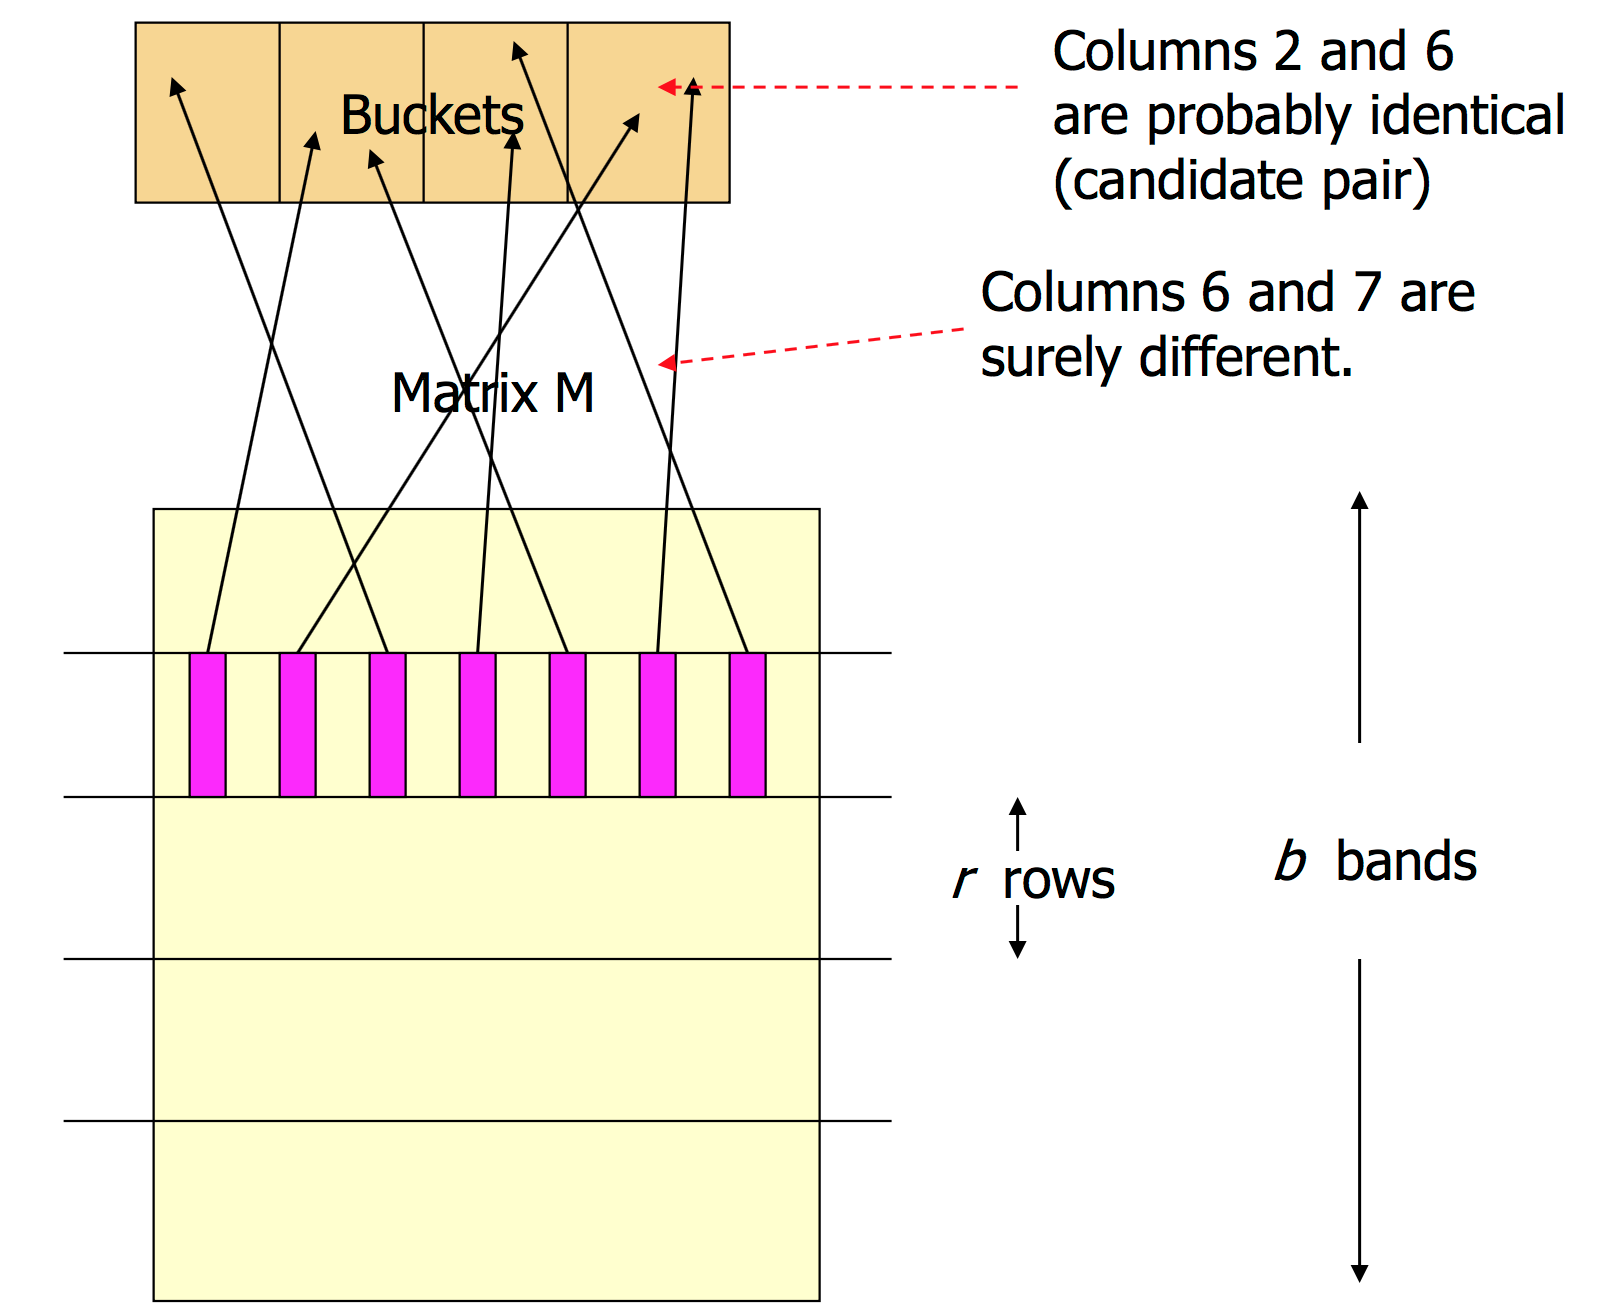
\includegraphics[width=9cm]{hashing-bands}

\end{frame}

%%%%%
  
\begin{frame} \frametitle{Simplifying Assumption}

There are enough buckets that columns are unlikely to hash to the same bucket unless they are identical in a particular band
Hereafter, we assume that \emph{same bucket} means \emph{identical in that band}
Assumption needed only to simplify analysis, not for correctness of algorithm

\end{frame}

%%%%%
  
\begin{frame} \frametitle{Example of Bands (1)}

Assume the following case:
  Suppose 100,000 columns of M (100k docs)
  Signatures of 100 integers (rows)
  Therefore, signatures take 40Mb
  Choose 20 bands of 5 integers/band
Goal: Find pairs of documents that are at least s = 80\% similar

\end{frame}

%%%%%
  
\begin{frame} \frametitle{Example of Bands (2)}

Assume: C1, C2 are 80\% similar
Since s=80% we want C1, C2 to hash to at least one common bucket (at least one band is identical)
Probability C1, C2 identical in one particular band: $(0.8)^5 = 0.328$
Probability C1, C2 are not similar in all of the 20 bands: $(1-0.328)^{20} = 0.00035$
  i.e., about 1/3000th of the 80\%-similar column pairs are false negatives
  We would find 99.965\% pairs of truly similar documents
  
\end{frame}

%%%%%
  
\begin{frame} \frametitle{Example of Bands (3)}

Assume: C1, C2 are 30\% similar
Since s=80% we want C1, C2 to hash to at NO common buckets (all bands should be different)
Probability C1, C2 identical in one particular band: $(0.3)^5 = 0.00243$
Probability C1, C2 identical in at least 1 of 20 bands: $1 - (1 - 0.00243)^{20} = 0.0474$
  In other words, approximately 4.74\% pairs of docs with similarity 30\% end up becoming candidate pairs -- false positives
  
\end{frame}

%%%%%
  
\begin{frame} \frametitle{LSH Involves a Tradeoff}

Pick:
  the number of minhashes (rows of M)
  the number of bands b, and
  the number of rows r per band
to balance false positives/negatives
Example: if we had only 15 bands of 5 rows, the number of false positives would go down, but the number of false negatives would go up

\end{frame}

%%%%%
  
\begin{frame} \frametitle{Analysis of LSH - What We Want}

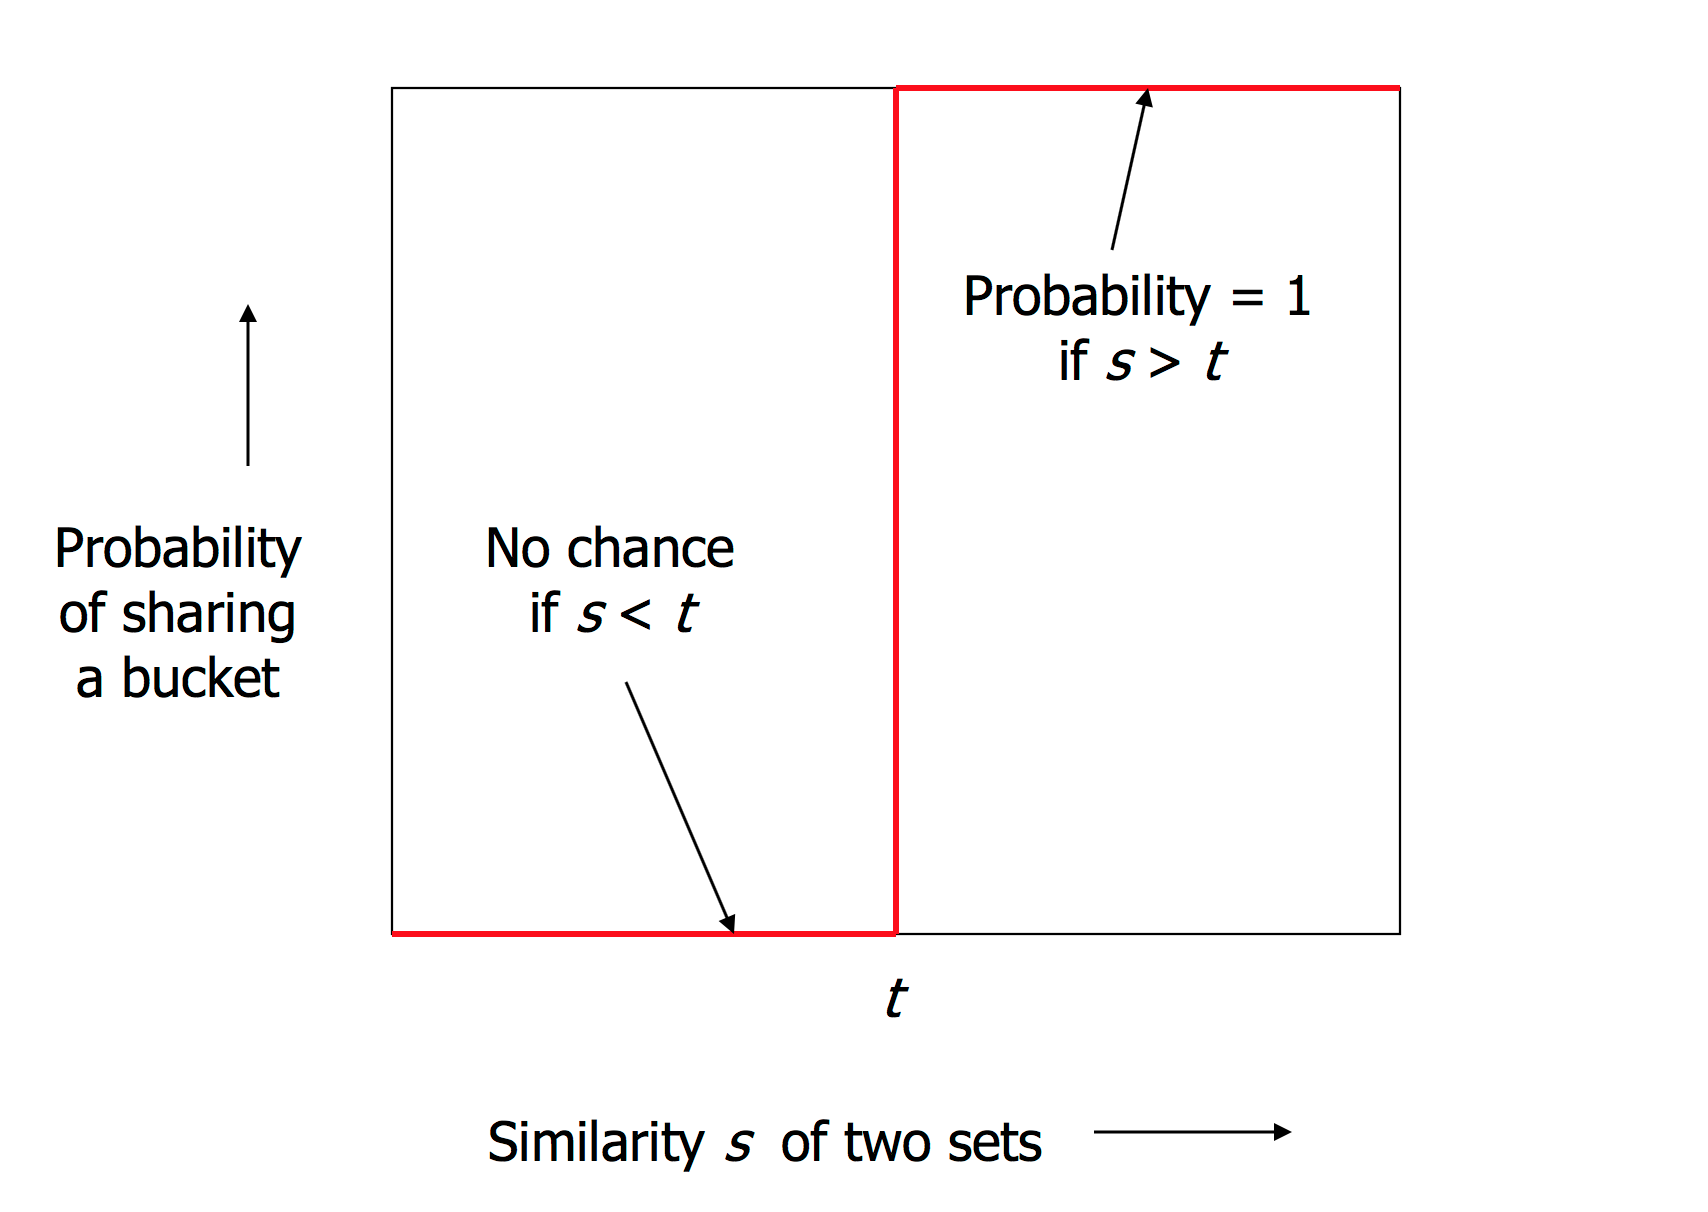
\includegraphics[width=10cm]{what-we-want}

\end{frame}

%%%%%
  
\begin{frame} \frametitle{Analysis of LSH - What One Band With One Row Gives}

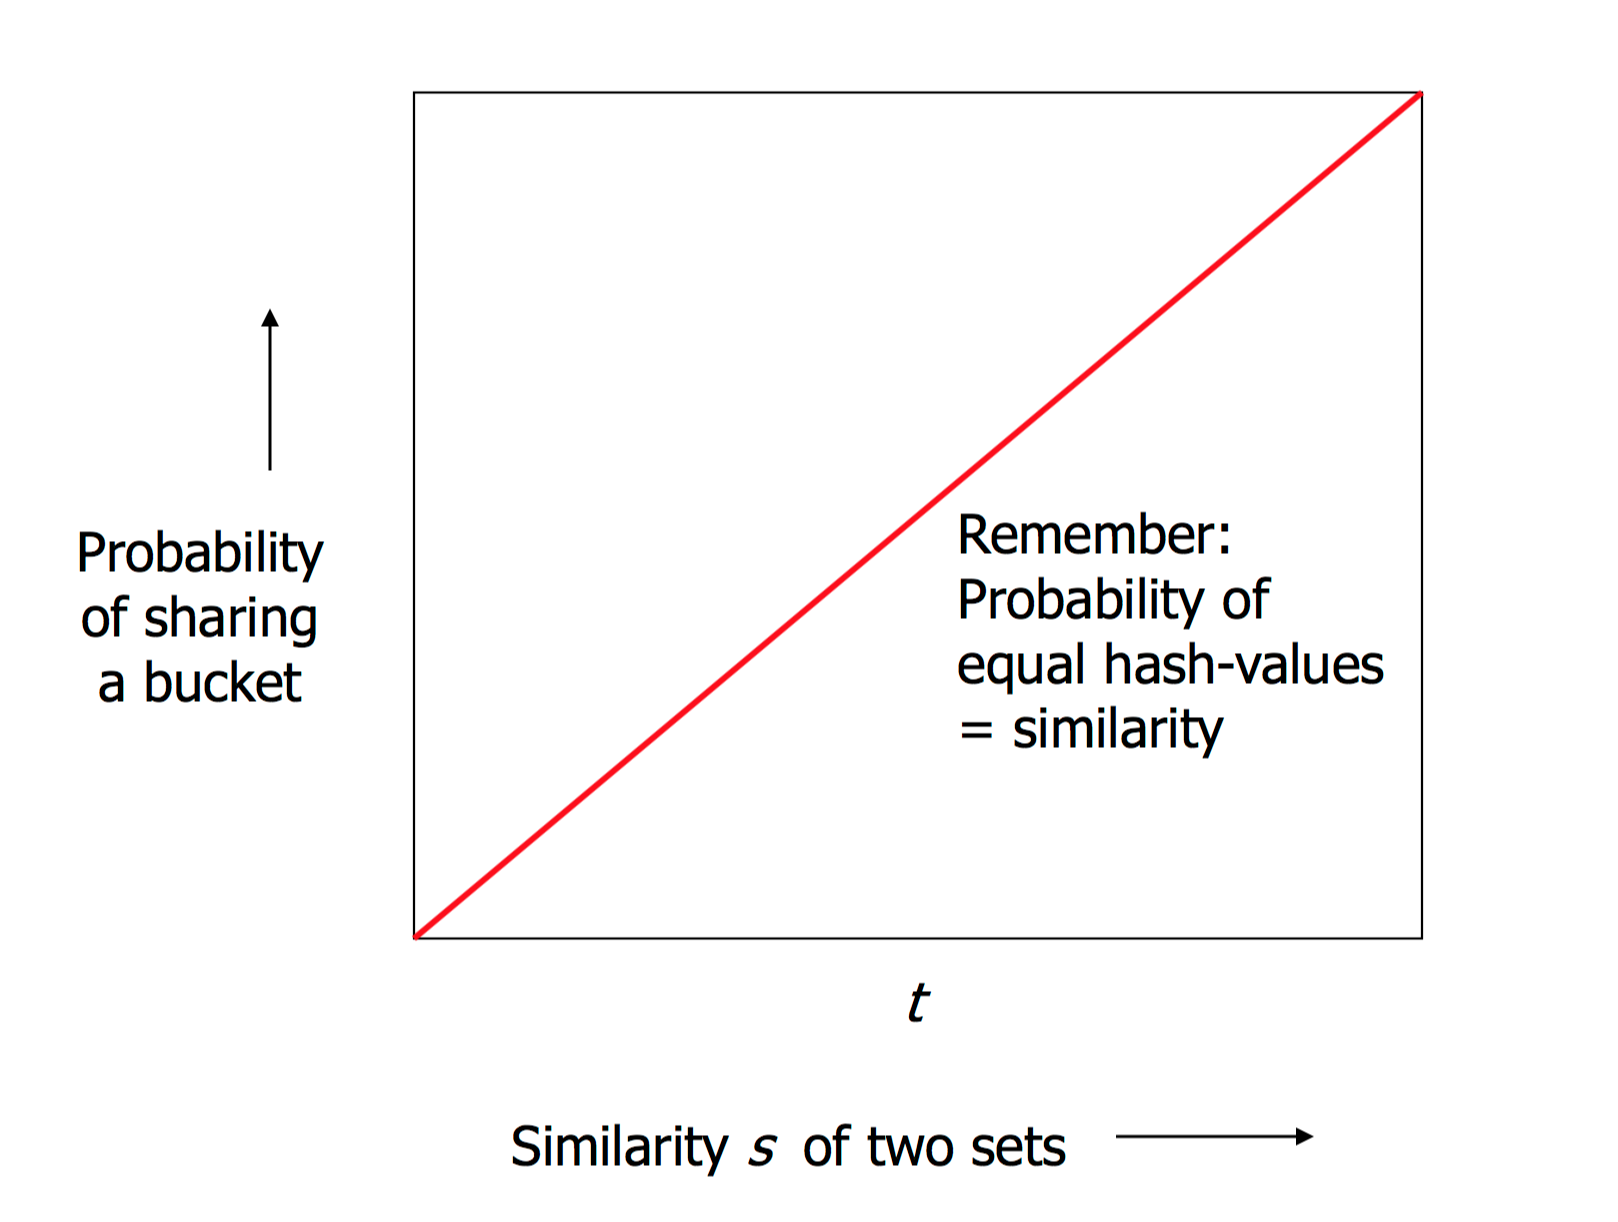
\includegraphics[width=10cm]{what-1-band-gives}

\end{frame}

%%%%%
  
\begin{frame} \frametitle{Analysis of LSH - b bands with b rows/band}

Columns $C_1$ and $C_2$ have similarity $s$
Pick any band (r rows)
  Prob. that all rows in band equal = $s^r$
  Prob. that some row in band unequal = $1 - s^r$
  Prob. that no band identical = $(1 - s^r)^b$
  Prob. that at least 1 band identical = $1 - (1 - s^r)^b$  
\end{frame}

%%%%%
  
\begin{frame} \frametitle{Analysis of LSH - What b Bands With r Rows Gives}

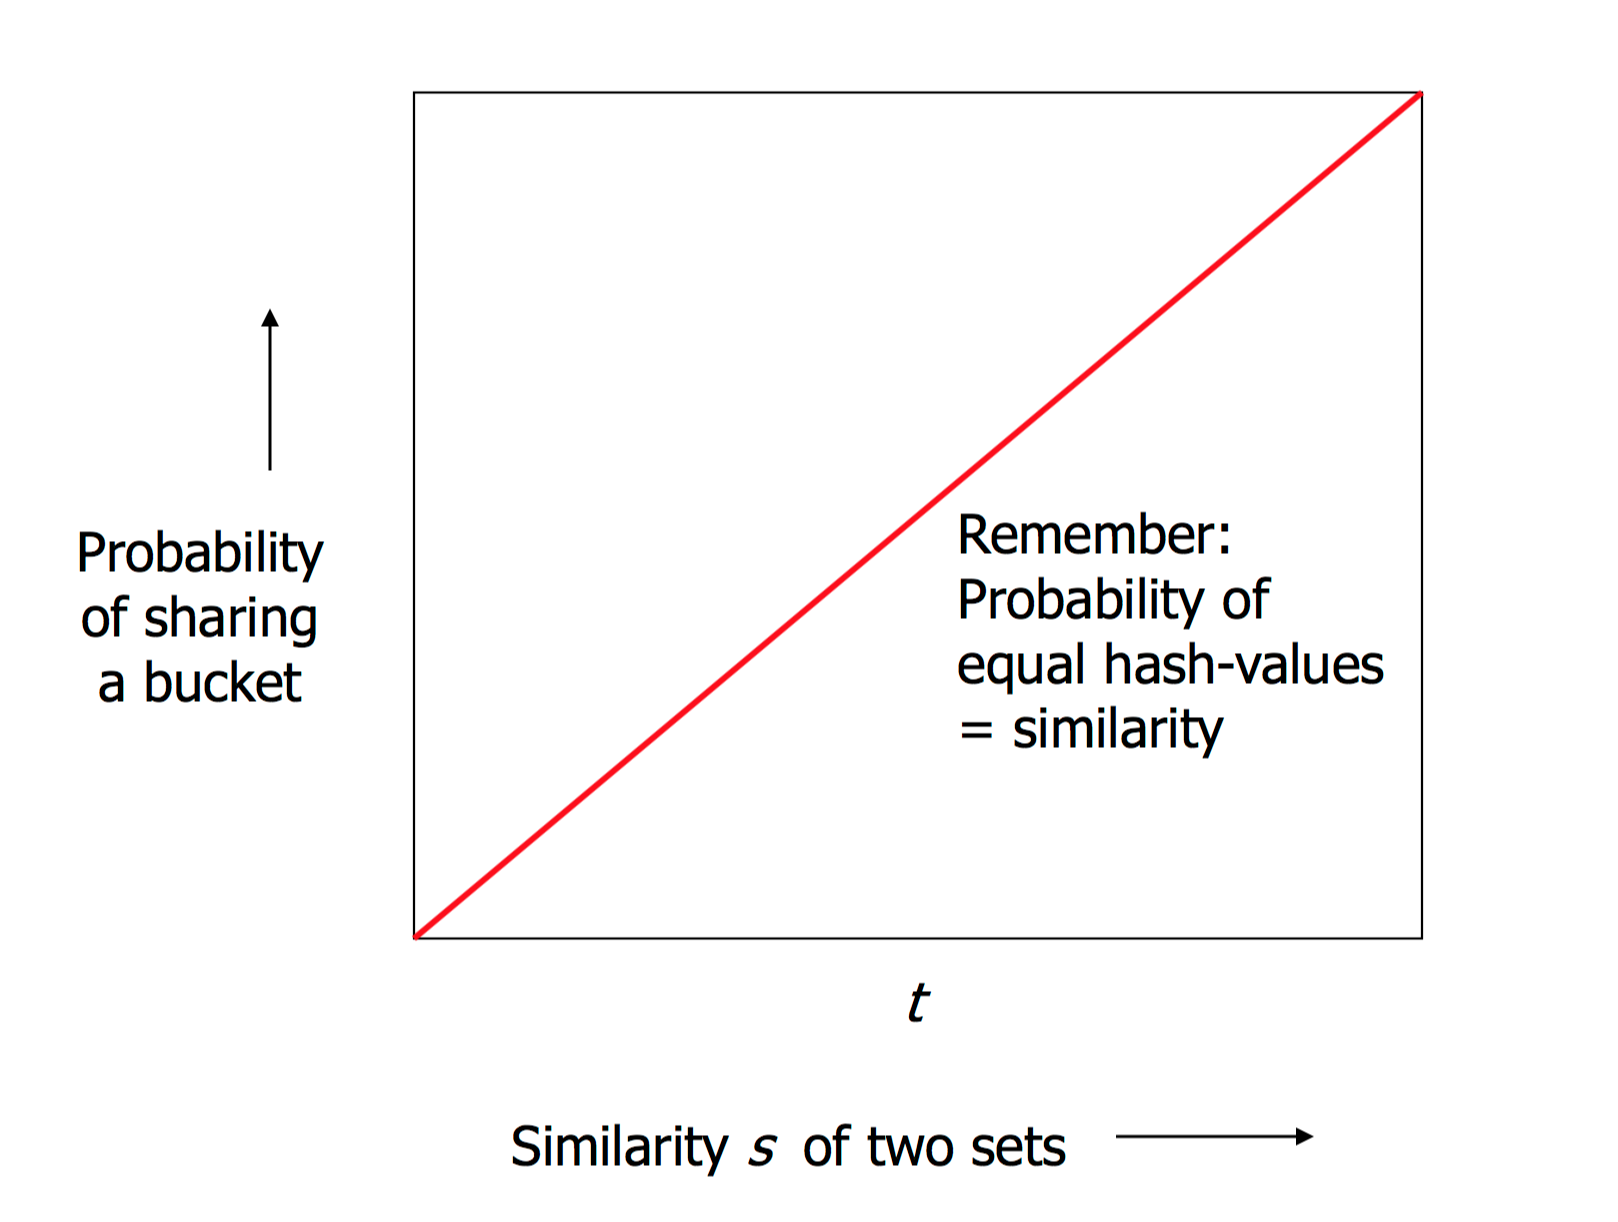
\includegraphics[width=10cm]{what-1-band-gives}

\end{frame}

%%%%%
  
\begin{frame} \frametitle{False Positives vs. False Negatives}

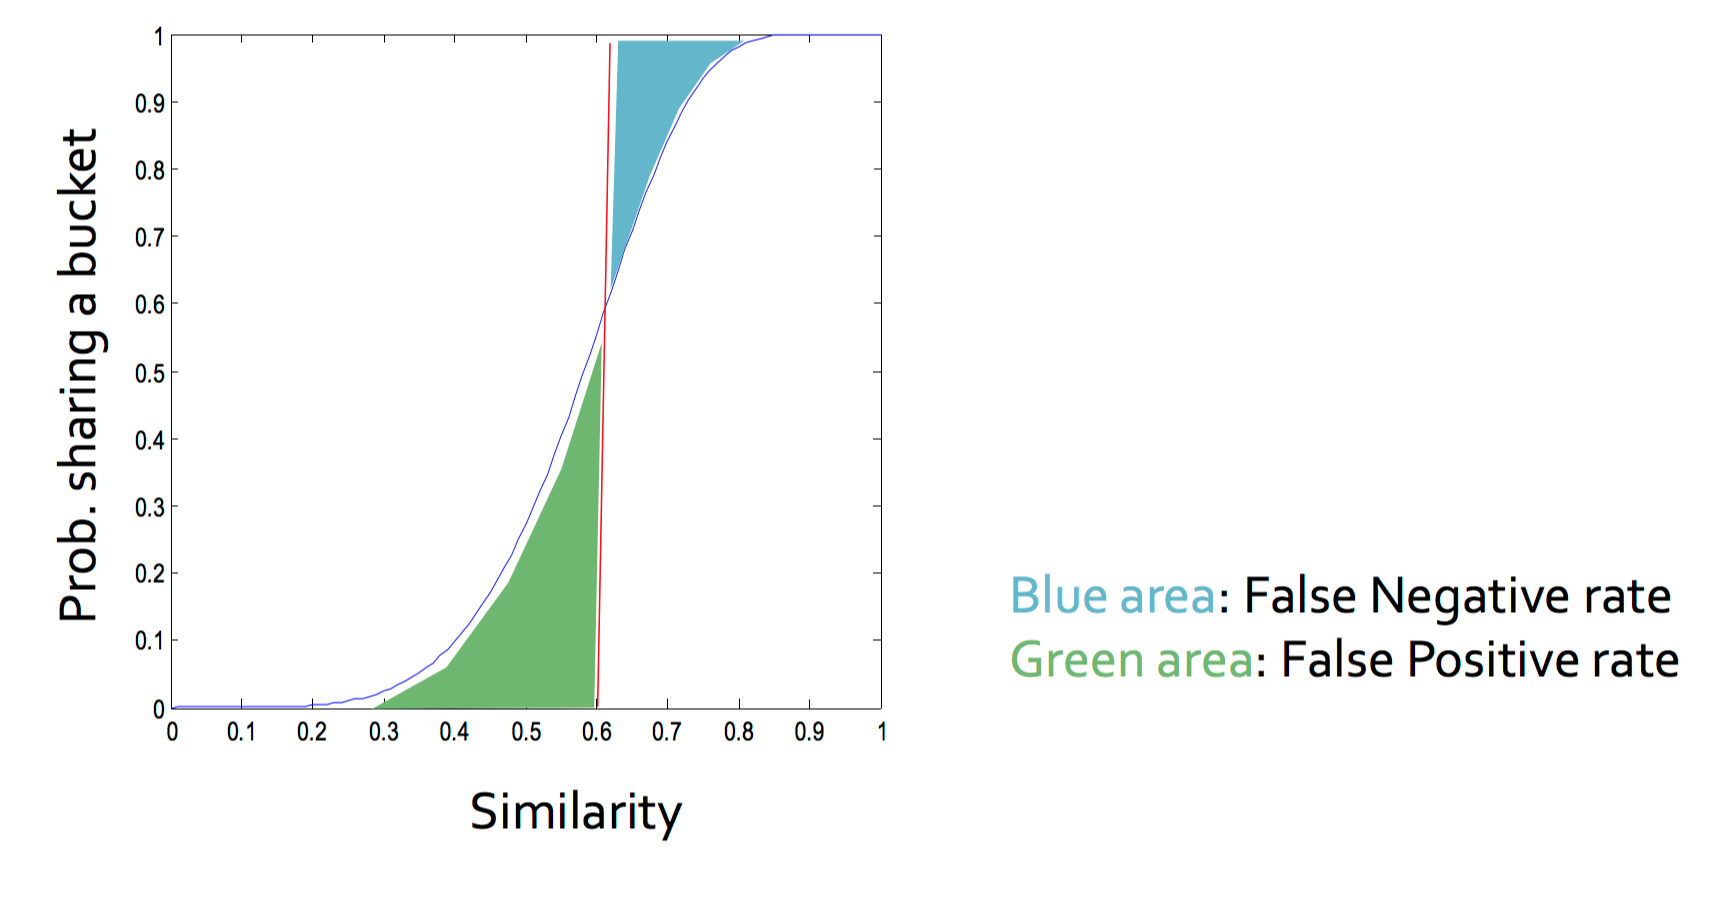
\includegraphics[width=10cm]{tradeoff}

\end{frame}

%%%%%
  
\begin{frame} \frametitle{LSH Summary}

Tune to get almost all pairs with similar signatures, but eliminate most pairs that do not have similar signatures
Check in main memory that candidate pairs really do have similar signatures
Optional: In another pass through data, check that the remaining candidate pairs really represent similar documents

\end{frame}

%%%%%
  
\begin{frame} \frametitle{The Big Picture}

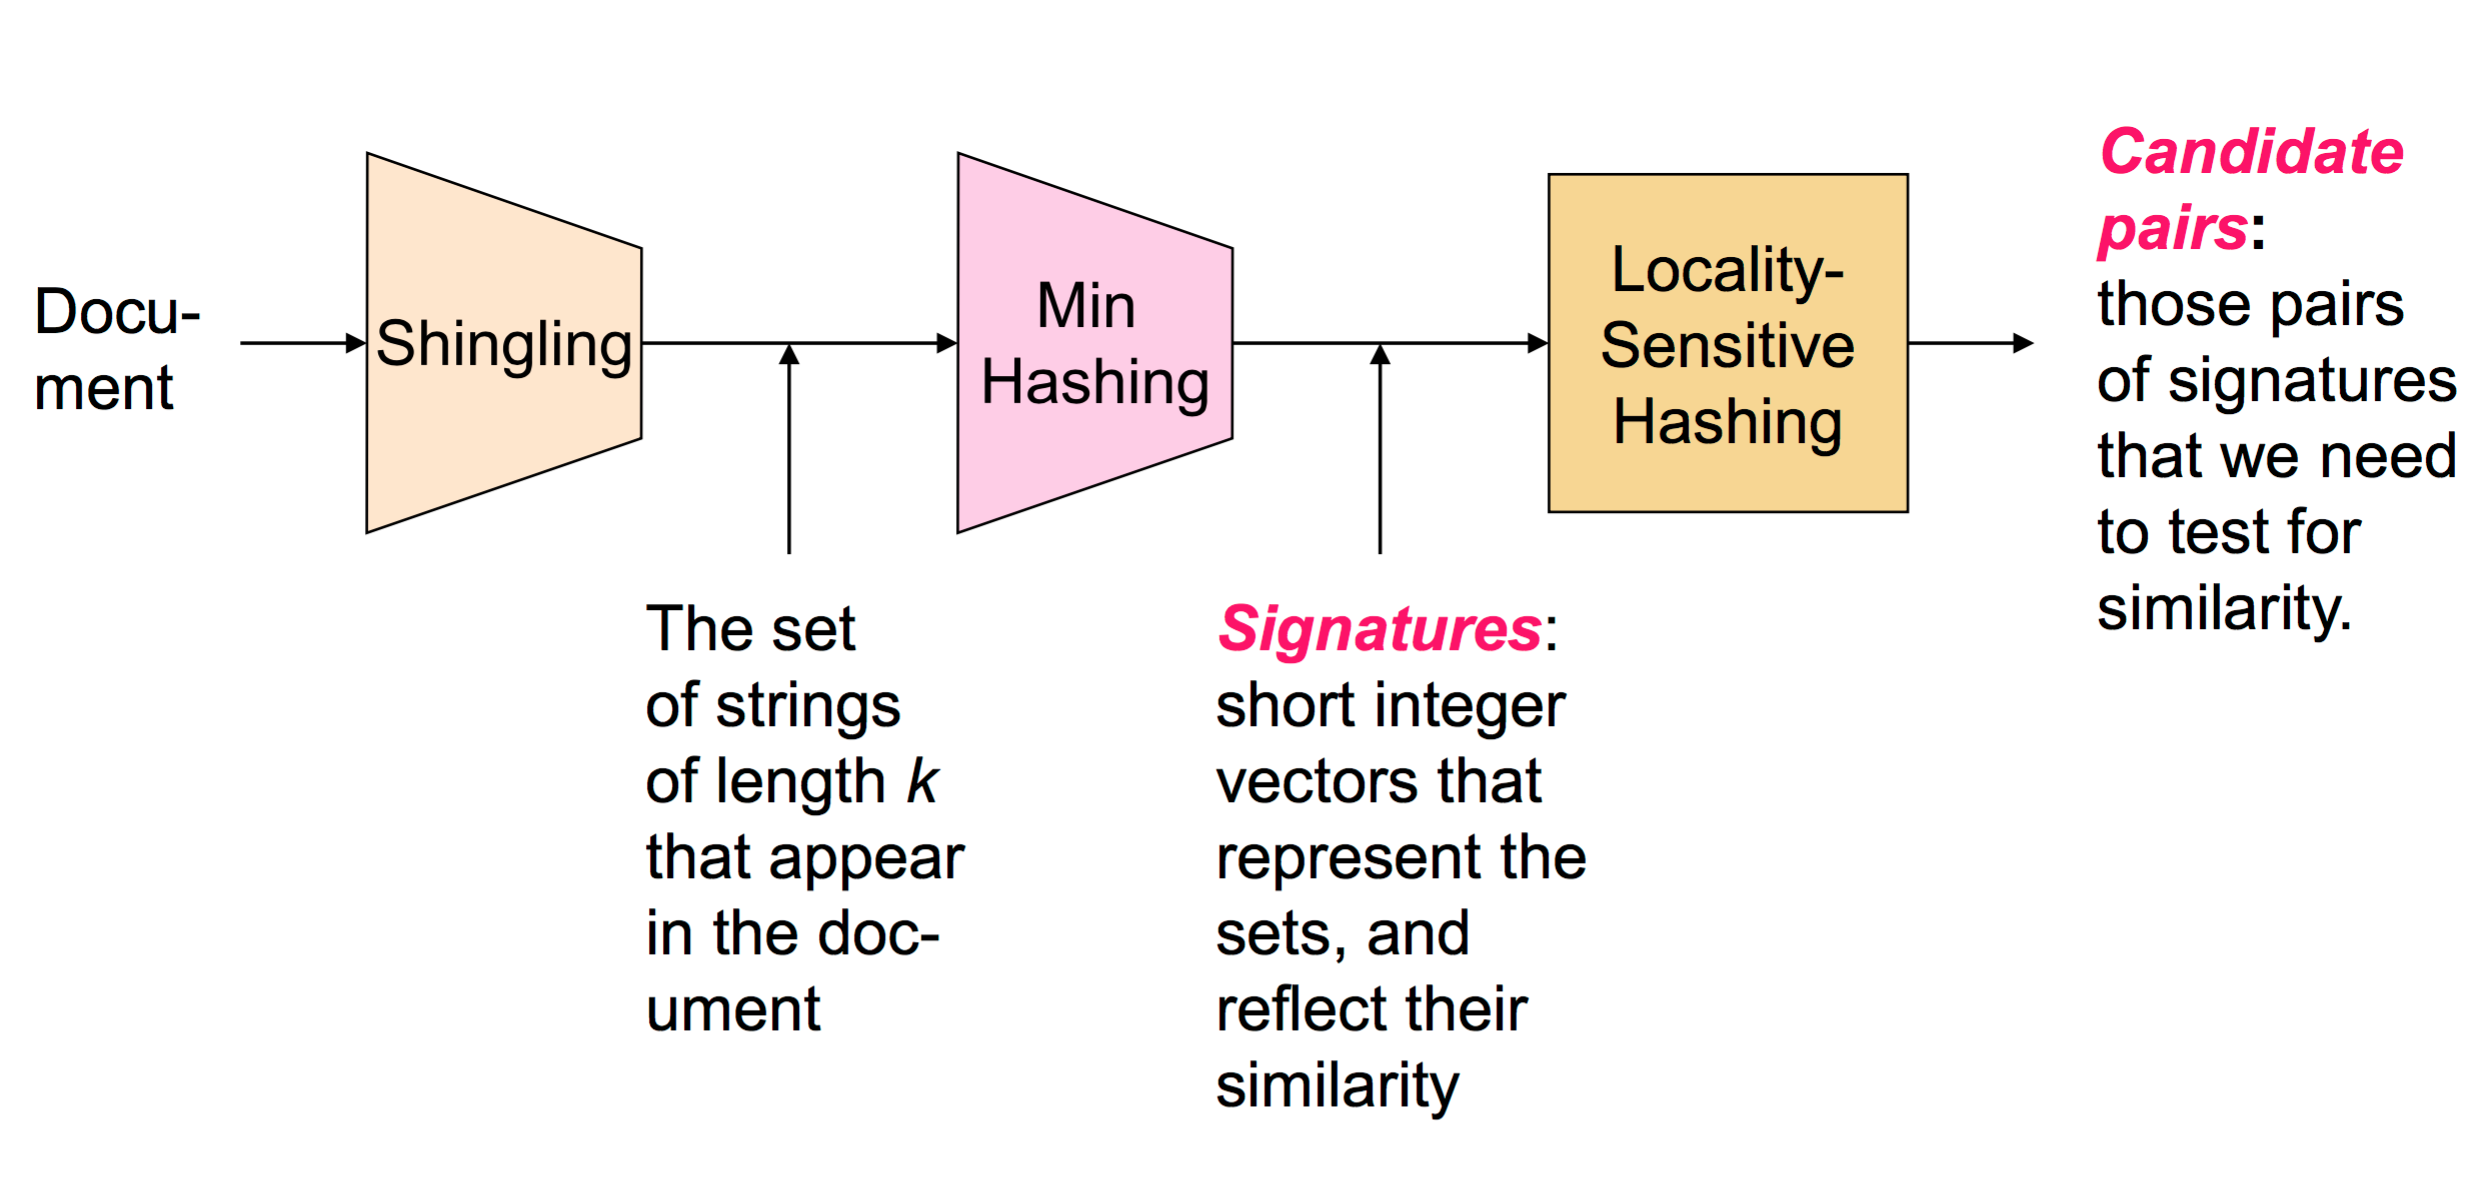
\includegraphics[width=10cm]{overall}

\end{frame}

%%%%%

\finalframe{Questions?}

\end{document}
